\documentclass[a4paper]{article}

% Basic packages
\usepackage{fontspec}
\XeTeXlinebreaklocale "zh"    % 启用中文断行（XeTeX 内建，无需 xeCJK）
\XeTeXlinebreakskip = 0pt plus 1pt
\setmainfont{Songti SC}
\setsansfont{Heiti SC}
\setmonofont{Menlo}
\usepackage{amsmath, amssymb}
\usepackage{graphicx}
\usepackage[margin=2.5cm]{geometry}
\usepackage[most]{tcolorbox}
\usepackage{etoolbox}
\usepackage{listings}
\usepackage{hyperref}
\usepackage{booktabs}
\usepackage{subcaption}
\usepackage{float}

% Chinese font setup (macOS system fonts, no ctex needed)
\setmainfont{Songti SC}
\setsansfont{Heiti SC}
\setmonofont{Menlo}
\newcommand{\song}{\fontspec{Songti SC}}
\newcommand{\hei}{\fontspec{Heiti SC}}
\newcommand{\kai}{\fontspec{KaiTi}}
\newcommand{\fangsong}{\fontspec{FangSong}}

% ===== Highlight boxes =====
\newtcolorbox{knowledgebox}[1]{
    enhanced, colback=blue!5!white, colframe=blue!75!black, colbacktitle=blue!75!black,
    coltitle=white, fonttitle=\bfseries, title=#1, attach boxed title to top left={yshift=-2mm, xshift=2mm},
    boxrule=1pt, sharp corners
}

\newtcolorbox{importantbox}[1]{
    enhanced, colback=yellow!10!white, colframe=yellow!80!black, colbacktitle=yellow!80!black,
    coltitle=black, fonttitle=\bfseries, title=#1, sharp corners
}

\newtcolorbox{warningbox}[1]{
    enhanced, colback=red!5!white, colframe=red!75!black, colbacktitle=red!75!black,
    coltitle=white, fonttitle=\bfseries, title=#1, sharp corners
}

\newtcolorbox{practicebox}[1]{
    enhanced, colback=green!5!white, colframe=green!60!black, colbacktitle=green!60!black,
    coltitle=white, fonttitle=\bfseries, title=#1, sharp corners
}

% ===== Code listings =====
\lstset{
    basicstyle=\ttfamily\small,
    keywordstyle=\color{blue},
    stringstyle=\color{red!60!black},
    commentstyle=\color{green!60!black},
    breaklines=true,
    frame=single,
    numbers=left,
    numberstyle=\tiny\color{gray},
    captionpos=b,
    extendedchars=false
}

% ===== Front-page metadata =====
\newcommand{\notetitle}{CS336 Lecture 4：Mixture of Experts}
\newcommand{\notesubtitle}{Stanford CS336: Language Modeling from Scratch (Spring 2025)}
\newcommand{\noteauthors}{讲师：Percy Liang, Tatsu Hashimoto \quad 笔记：ZCode}
\newcommand{\notedate}{2026-07-14}
\newcommand{\videochannel}{Stanford CS336}
\newcommand{\videopublishdate}{2025 Spring}
\newcommand{\videoduration}{82 分钟}
\newcommand{\videourl}{https://www.youtube.com/watch?v=LPv1KfUXLCo}
\newcommand{\videocoverpath}{cover.jpg}

\begin{document}

% ===== Title page =====
\begin{titlepage}
\centering
{\Large 课程笔记\par}
\vspace{1.2cm}
{\huge\bfseries \notetitle\par}
\vspace{0.3cm}
{\large \notesubtitle\par}
\vspace{0.5cm}
{\large \noteauthors\par}
\vspace{0.3cm}
{\large \notedate\par}
\vspace{1.0cm}

\includegraphics[width=0.82\textwidth,height=0.40\textheight,keepaspectratio]{\videocoverpath}\par

\vfill
\begin{tcolorbox}[width=0.9\textwidth, colback=black!2!white, colframe=black!60, sharp corners]
\textbf{视频作者/频道}：\videochannel\par
\textbf{发布日期}：\videopublishdate\par
\textbf{视频时长}：\videoduration\par
\textbf{视频链接}：\href{\videourl}{\nolinkurl{\videourl}}
\end{tcolorbox}
\end{titlepage}

\tableofcontents
\newpage

%% --- 正文内容开始 ---

\section{导论：为什么 MoE 成了主流}

\subsection{从 DeepSeek V3 说起：本讲动机}

本讲聚焦于 Mixture of Experts（混合专家，简称 MoE）。Percy Liang 开篇即点题：如今几乎所有最前沿的大语言模型——DeepSeek V3、Grok、Qwen、Gemini——其核心架构都已转向 MoE。理解 DeepSeek V3 这一类模型，绕不开对 MoE 机制、训练技巧和工程权衡的深入掌握。

\begin{figure}[H]
\centering
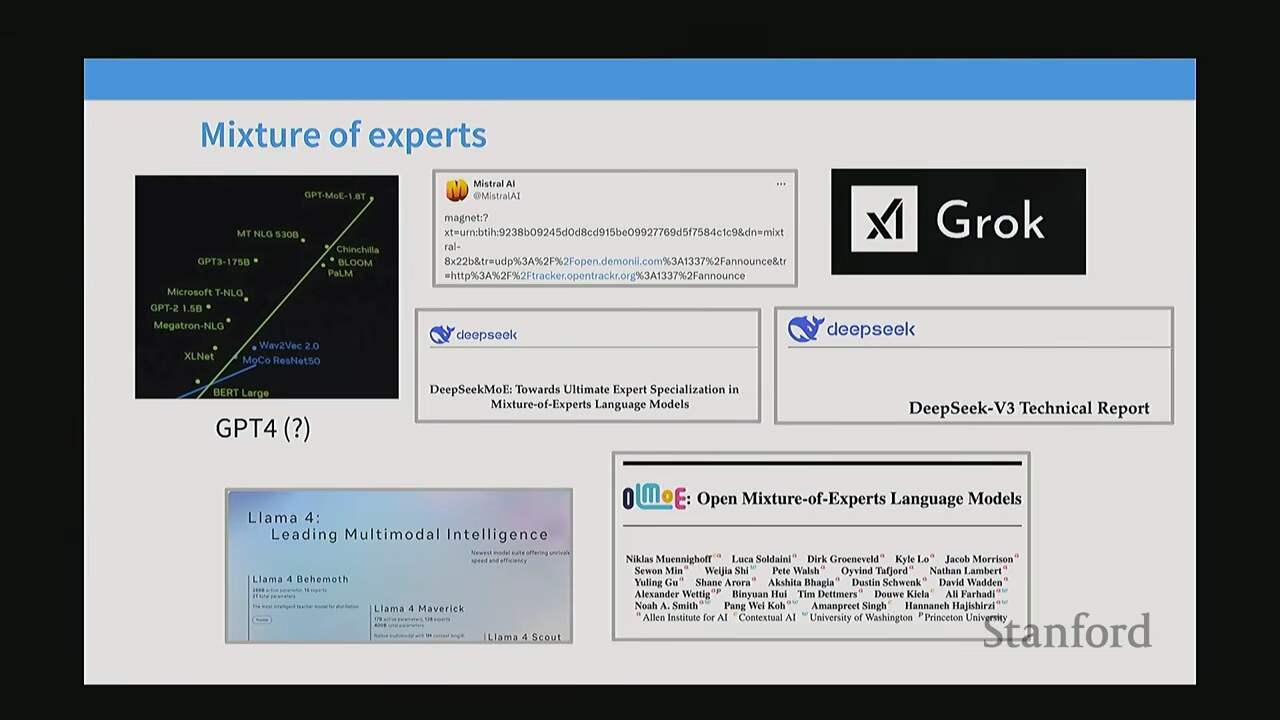
\includegraphics[width=\textwidth]{figures/fig_01_what_is_moe.jpg}
\caption{本讲开篇提纲：从"什么是 MoE"出发，覆盖路由、负载均衡、专家并行、训练稳定性以及 DeepSeek V2/V3 的具体设计\protect\footnotemark}
\end{figure}
\footnotetext{视频画面时间区间：00:00:45--00:01:15。}

\begin{importantbox}{核心问题}
\begin{itemize}
\item MoE 究竟解决了什么问题？为什么 sparse 模型能在相同训练算力下胜过 dense 模型？
\item router（路由器）是怎么"挑专家"的？这一操作和 attention 有何本质联系？
\item 训练 MoE 时最棘手的工程难题（routing collapse、负载不均、token dropping、通信开销）如何一一化解？
\item DeepSeek V3 真正的架构创新（auxiliary-loss-free balancing、MLA、MTP）是什么？
\end{itemize}
\end{importantbox}

\subsection{Sparse 相对 Dense 的根本优势}

Dense 模型里，每个 token 都要流过全部参数，参数量与每个 token 的计算量（FLOPs）线性绑定。MoE 打破了这一绑定：总参数可以做得很大，但每个 token 只激活其中一小部分专家，从而在固定推理/训练算力下塞进更多知识。

设 dense FFN 的参数量为 $P_{\text{dense}}$，MoE 有 $N$ 个专家、每个 token 激活 $k$ 个、单专家参数量为 $P_{\text{exp}}$，则：

\[
P_{\text{total}} \;=\; N \cdot P_{\text{exp}} \;+\; P_{\text{shared}}, \qquad P_{\text{active}} \;=\; k \cdot P_{\text{exp}} \;+\; P_{\text{shared}}
\]

\begin{itemize}
\item $P_{\text{total}}$：模型全部可学习参数（决定容量与显存）。
\item $P_{\text{active}}$：每个 token 实际激活的参数（决定单 token 的 FLOPs）。
\item MoE 的核心价值就是 $P_{\text{total}} \gg P_{\text{active}}$，把"总容量"与"单步算力"解耦。
\end{itemize}

训练效率可以用"每 FLOP 损失下降"来衡量：在相同总训练算力 $C$ 下，MoE 因参数更多能学到更复杂的函数，因而 loss 降得更低。这正是 sparse 相对 dense 的根本优势所在。

\begin{figure}[H]
\centering
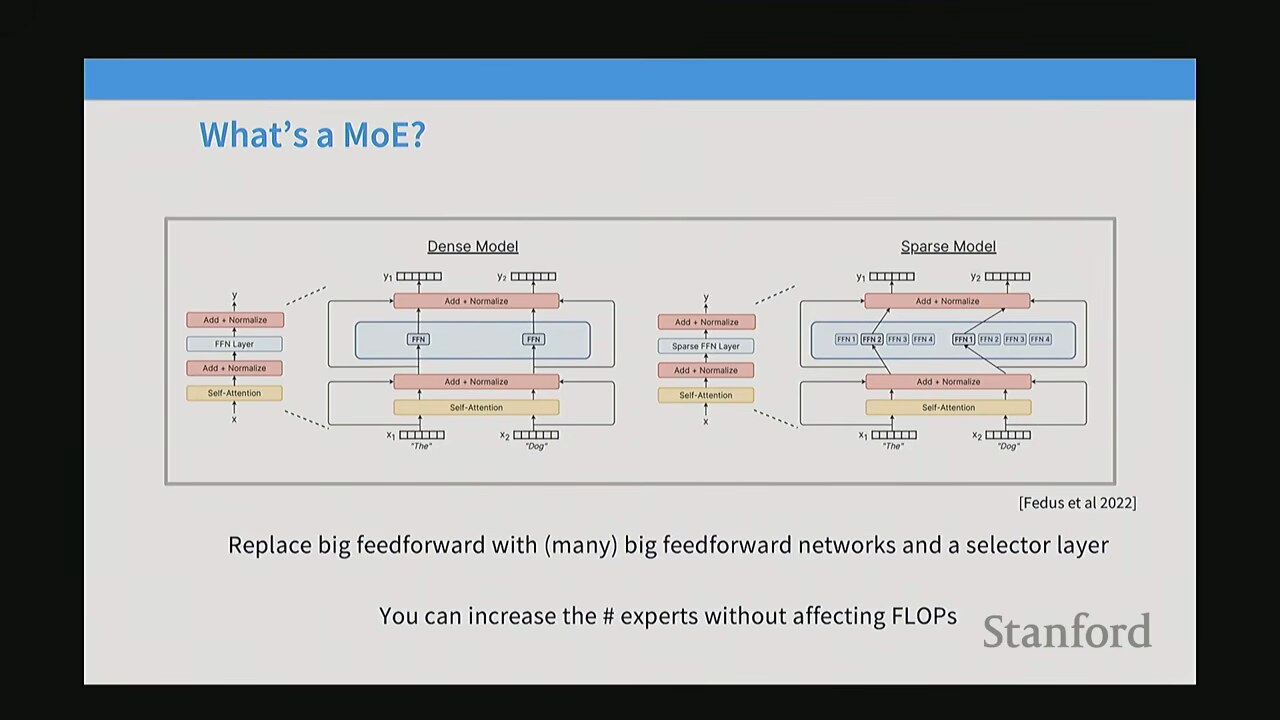
\includegraphics[width=\textwidth]{figures/fig_02_moe_motivation.jpg}
\caption{为什么需要 MoE：在相同训练算力预算下，sparse MoE 模型能取得比 dense 模型更低的 loss\protect\footnotemark}
\end{figure}
\footnotetext{视频画面时间区间：00:01:45--00:02:15。}

\begin{figure}[H]
\centering
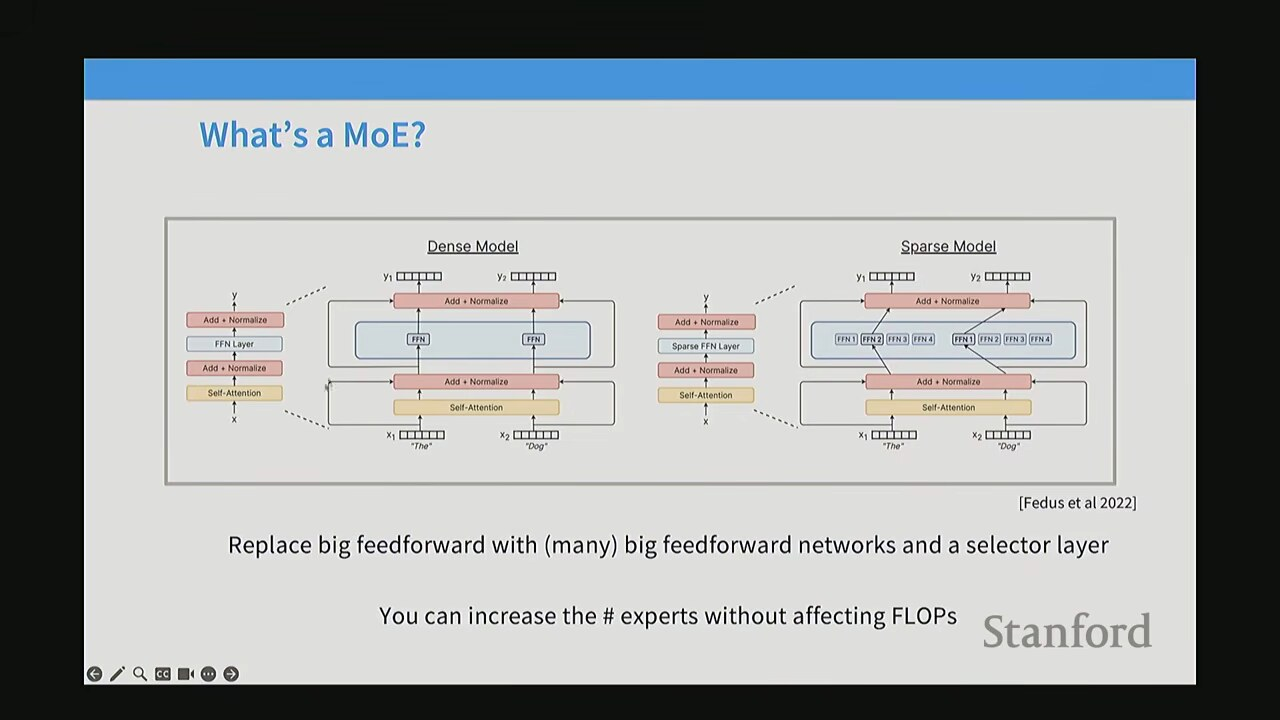
\includegraphics[width=\textwidth]{figures/fig_03_moe_definition.jpg}
\caption{MoE 是 conditional computation（条件计算）的一种形式：参数被稀疏激活，按输入动态选择\protect\footnotemark}
\end{figure}
\footnotetext{视频画面时间区间：00:02:15--00:02:45。}

\begin{knowledgebox}{关键术语：Conditional Computation}
Conditional computation（条件计算）指模型的计算图依据输入动态变化——不同的输入走不同的子网络分支。MoE 是其最成功的大规模实例：一个 router 决定每个 token 激活哪些专家子网络，使得"总容量"与"单次计算量"解耦。
\end{knowledgebox}

\section{MoE 的基本结构}

\subsection{Dense FFN vs Sparse MoE：并排对比}

在一个标准 Transformer block 里，self-attention 之后跟着一个 feed-forward network（FFN）。Dense 模型的 FFN 是"一整块"；而 sparse MoE 模型则把这块 FFN 替换成"一个 router + 若干并行的专家 FFN"。

\begin{figure}[H]
\centering
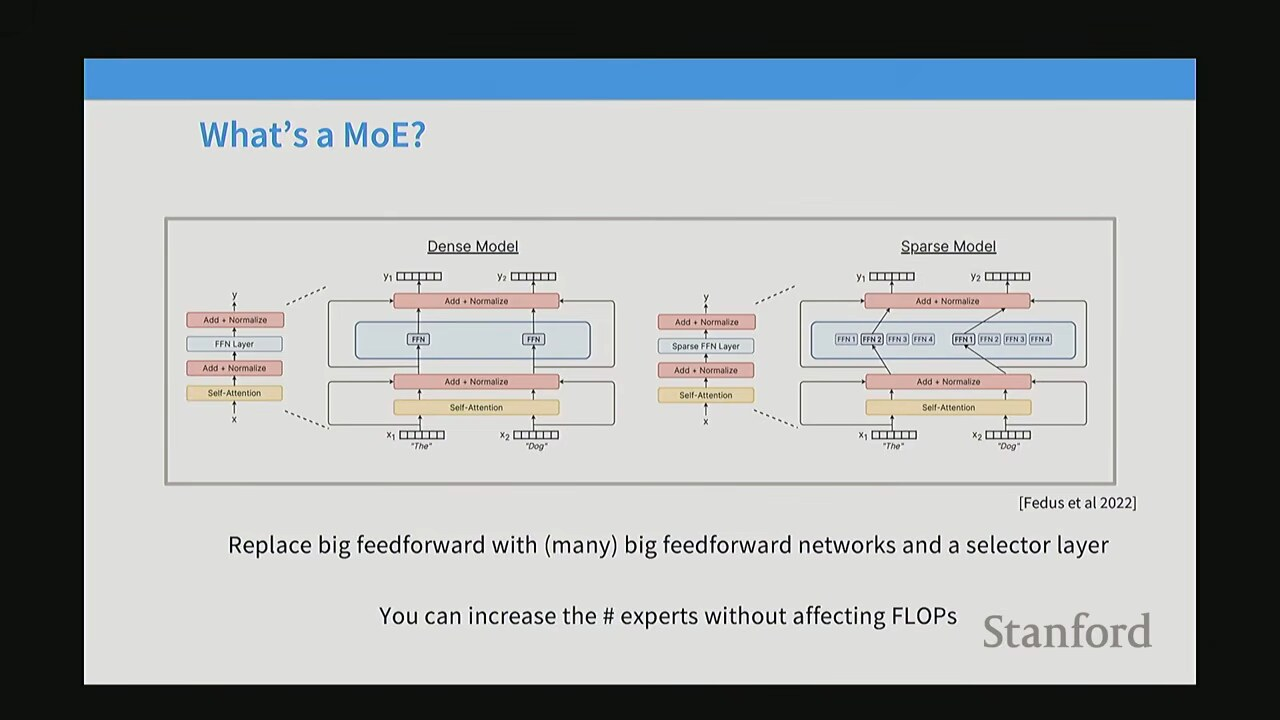
\includegraphics[width=\textwidth]{figures/fig_04_dense_vs_sparse.jpg}
\caption{Dense 模型与 Sparse MoE 模型的结构并排：左侧 dense 是一整块 FFN，右侧 sparse 用一个 selector/router 层加多个并行专家（Fedus et al., 2022）\protect\footnotemark}
\end{figure}
\footnotetext{视频画面时间区间：00:03:15--00:03:45。}

关键直觉：如果把 sparse 模型里所有被激活的专家加起来，其总宽度大致等于那个 dense FFN 的宽度，那么"每个 token 实际计算量"和 dense 模型相当；但可学习的总参数量却成倍增加。这正是 MoE 高效的根源。

\begin{figure}[H]
\centering
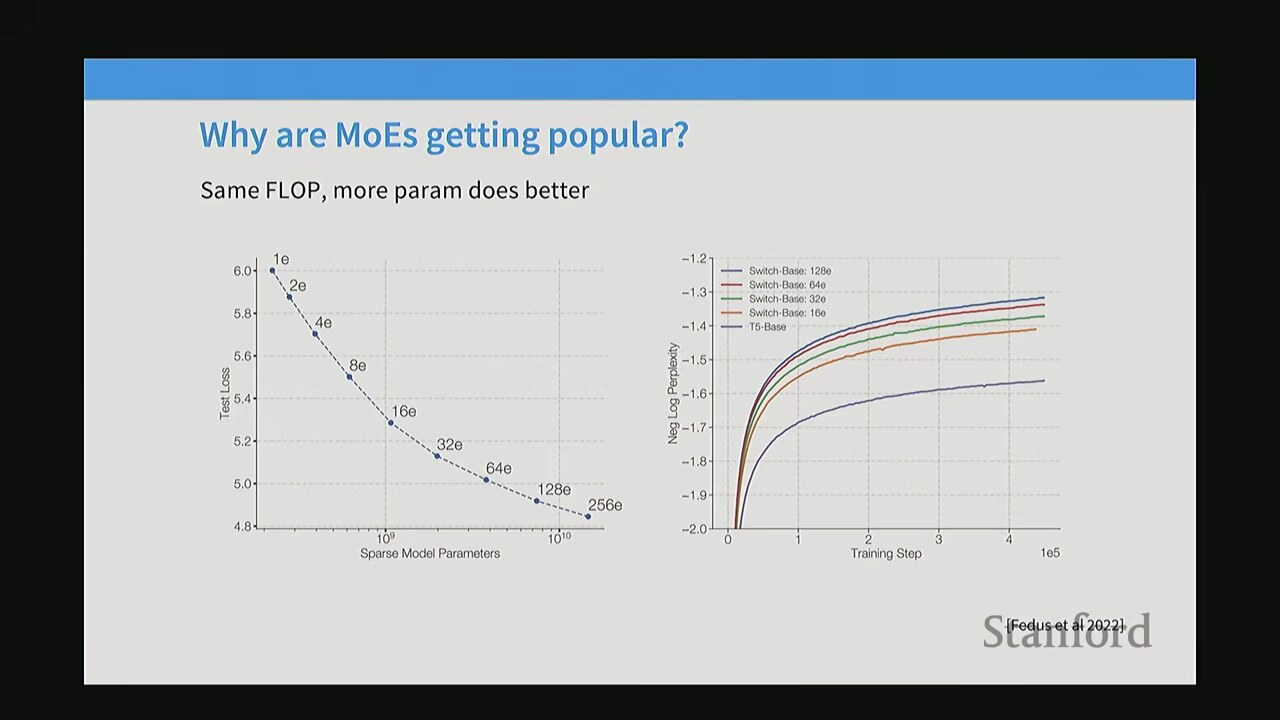
\includegraphics[width=\textwidth]{figures/fig_05_dense_vs_sparse_loss.jpg}
\caption{Dense 与 Sparse 模型在相同训练算力下的 loss 曲线对比：sparse 模型更快下降到更低水平\protect\footnotemark}
\end{figure}
\footnotetext{视频画面时间区间：00:03:45--00:04:15。}

\subsection{MoE 的性能实证：DeepSeek V2 与同侪}

Percy 展示了一组对比：在相近训练算力下，sparse MoE 架构（如 DeepSeek V2）能用远少于 dense 模型的激活参数，达到甚至超越后者的性能。

\begin{figure}[H]
\centering
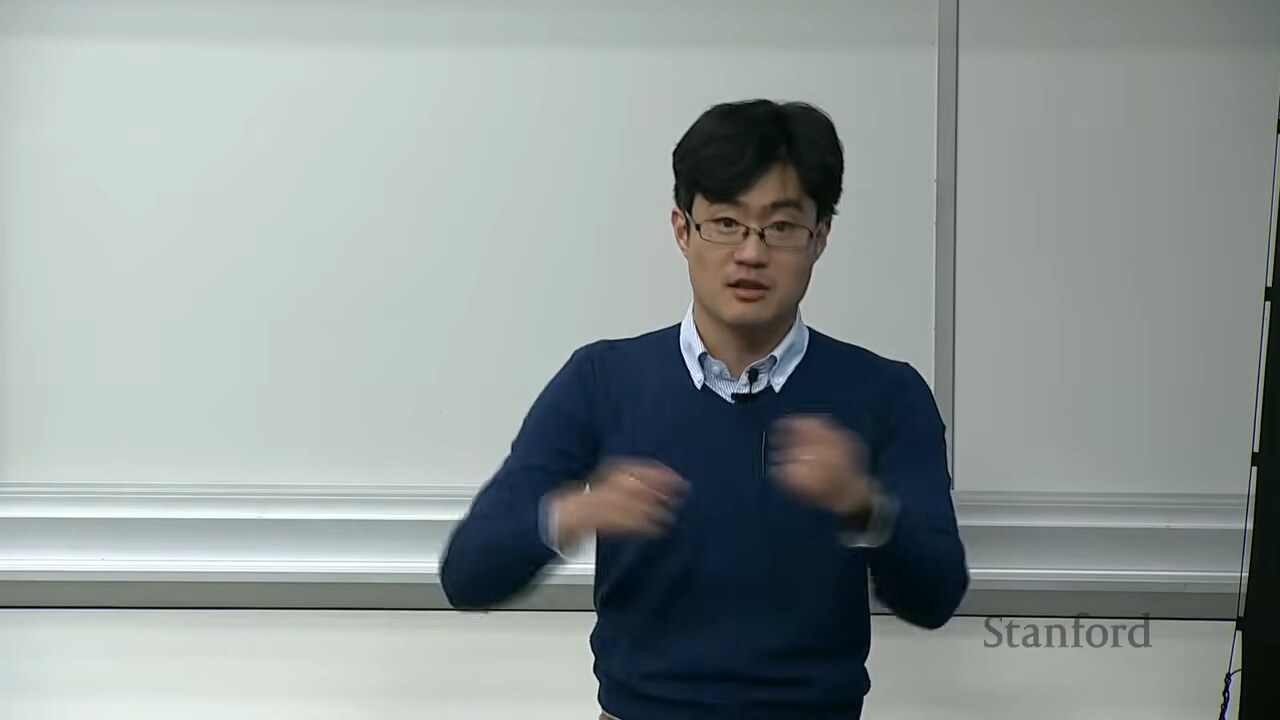
\includegraphics[width=\textwidth]{figures/fig_06_deepseek_v2_perf.jpg}
\caption{DeepSeek V2 等模型在更少的激活参数下达到强劲性能，印证 sparse 架构的高效性\protect\footnotemark}
\end{figure}
\footnotetext{视频画面时间区间：00:06:45--00:07:15。}

\begin{knowledgebox}{几个里程碑 MoE 模型}
\begin{itemize}
\item \textbf{GShard}（Lepikhin et al., 2020）：把 MoE 引入大规模 Transformer，每层用 top-2 路由，按专家切分到不同设备。
\item \textbf{Switch Transformer}（Fedus et al., 2022）：简化为 top-1 路由，首次把 MoE 训练扩展到万亿参数级别。
\item \textbf{ST-MoE}：在路由稳定性与下游任务微调上做了改进。
\item \textbf{DeepSeek-MoE}：提出 fine-grained expert + shared expert，显著提升了专家专业化。
\end{itemize}
\end{knowledgebox}

\subsection{Expert Parallelism：把专家分布到不同设备}

因为每个 token 只走少数专家，自然可以把不同的专家放在不同的 GPU 上，每个设备只负责自己那份专家的计算。这就是 expert parallelism（专家并行），它让 MoE 可以在多机上高效横向扩展。

\begin{figure}[H]
\centering
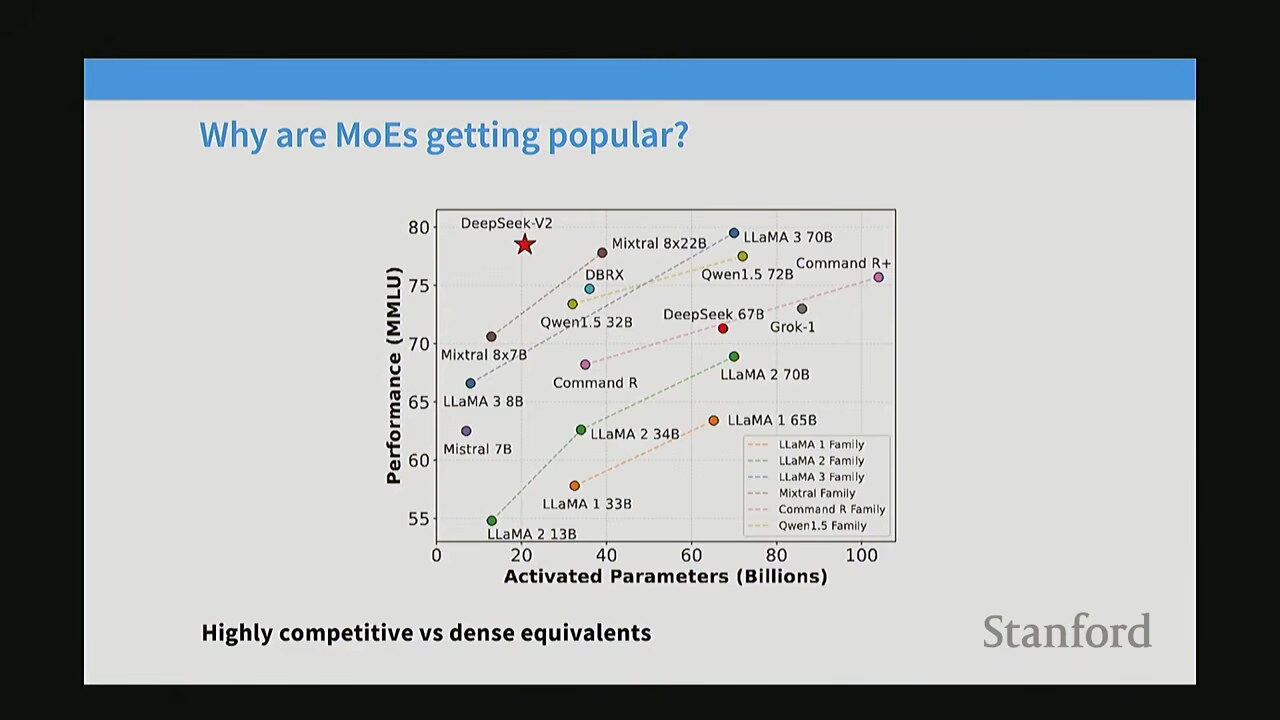
\includegraphics[width=\textwidth]{figures/fig_07_expert_parallel.jpg}
\caption{专家并行：不同专家分布在不同设备上，token 经路由后通过 all-to-all 通信发往对应设备\protect\footnotemark}
\end{figure}
\footnotetext{视频画面时间区间：00:07:15--00:07:45。}

\begin{warningbox}{为何 MoE 不像看起来那么"免费"}
虽然每个 token 只激活部分参数，但要训练一个总参数量巨大的 MoE，需要：足够的设备来容纳全部专家、跨设备的高效通信、以及专门设计的负载均衡损失。否则要么训练崩溃，要么通信开销吞掉稀疏化带来的收益。
\end{warningbox}

\subsection{Upcycling：从 Dense 模型"长出"MoE}

训练一个 MoE 从头开始成本高昂。Qwen 等团队提出了一个聪明的技巧：\textbf{upcycling}（上循环）——把一个已经训练好的 dense 模型的 FFN 权重复制 N 份，作为 N 个专家的初始化，再继续训练成 MoE。

\begin{figure}[H]
\centering
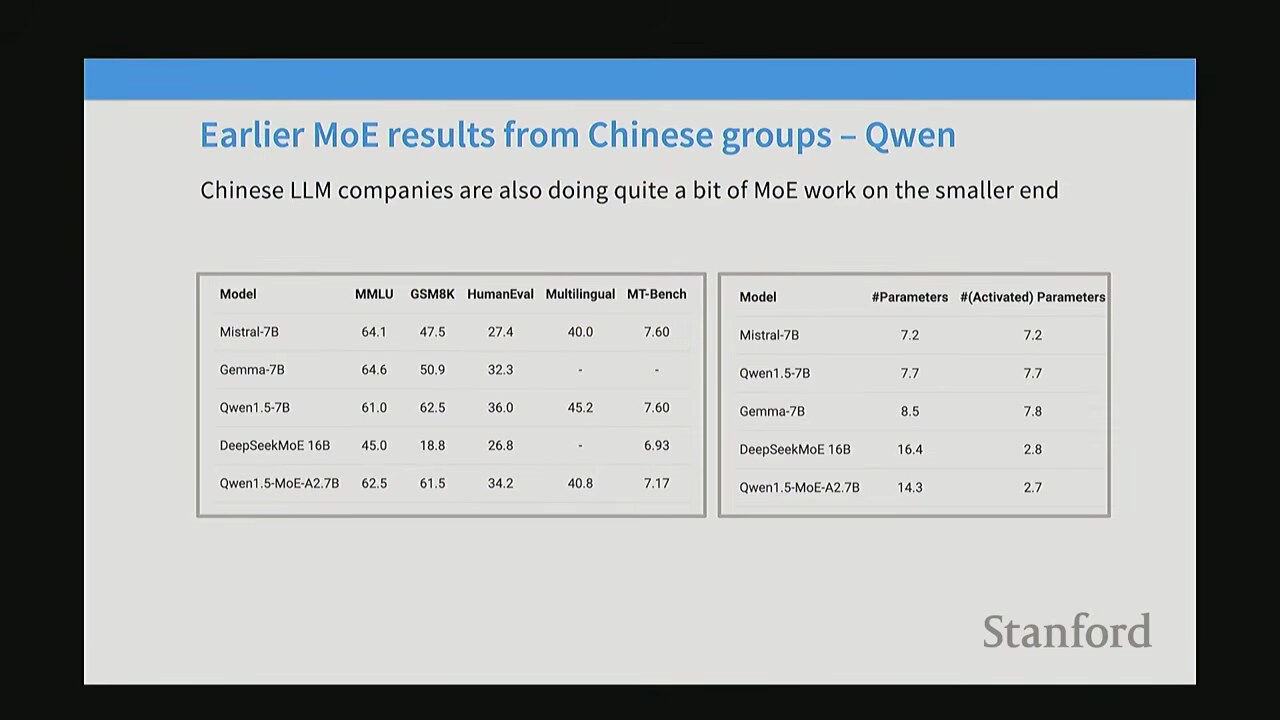
\includegraphics[width=\textwidth]{figures/fig_08_upcycling.jpg}
\caption{Upcycling 技巧：把 dense 模型的 FFN 权重切分/复制，初始化成 MoE 的多个专家（Qwen1.5 MoE 实例）\protect\footnotemark}
\end{figure}
\footnotetext{视频画面时间区间：00:09:45--00:10:15。}

\begin{practicebox}{工程启示}
Upcycling 让你能复用手头已有的 dense 模型，以较低成本获得一个 MoE 起点，而不必从零承担 MoE 训练的不稳定性。这是从 dense 走向 sparse 的一条务实路径。
\end{practicebox}

\section{路由机制：Router 如何挑专家}

\subsection{在哪里做稀疏化}

Transformer 一个 block 包含 attention 和 FFN。MoE 通常把 FFN 替换为稀疏专家层；理论上也可以做 sparsely-routed attention（稀疏注意力），但主流大模型（DeepSeek、Mixtral 等）都选择在 FFN 上稀疏化。

\begin{figure}[H]
\centering
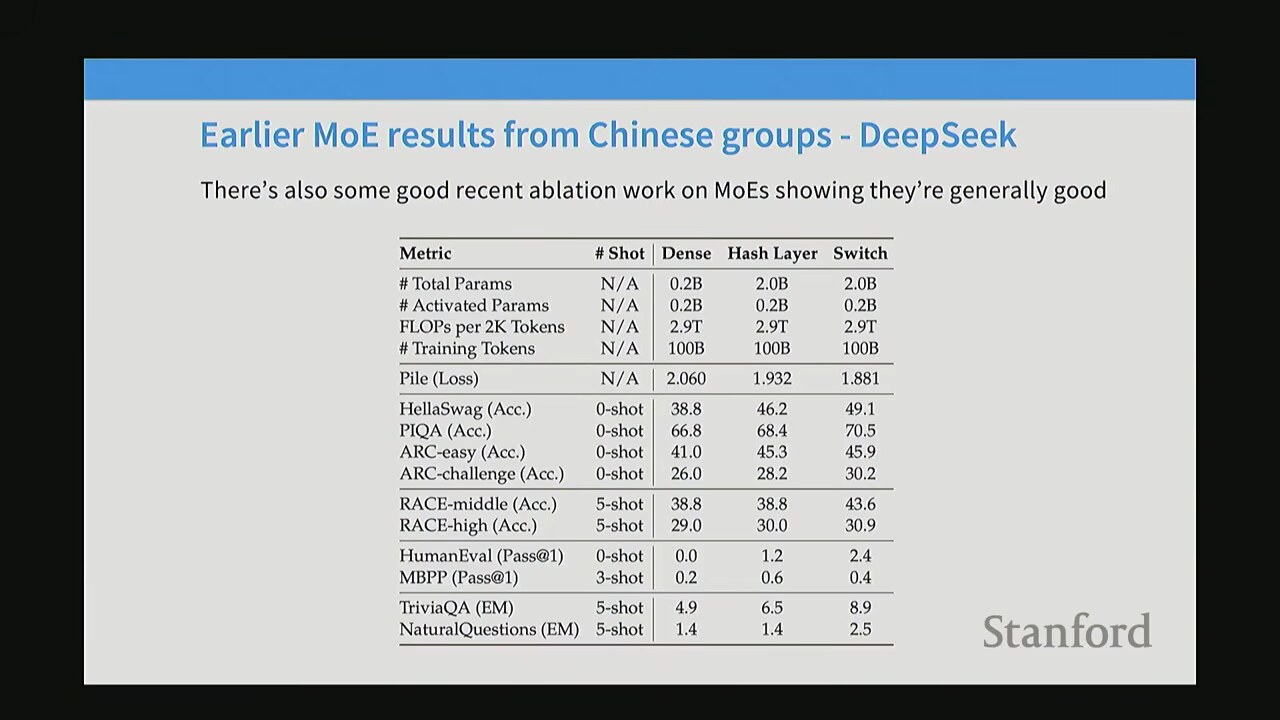
\includegraphics[width=\textwidth]{figures/fig_09_where_to_sparsify.jpg}
\caption{稀疏化的位置选择：通常替换 FFN 为 MoE，attention 也可做但非主流\protect\footnotemark}
\end{figure}
\footnotetext{视频画面时间区间：00:10:45--00:11:15。}

\subsection{Router 本质上就是一次 Attention}

Percy 反复强调一个深刻洞见：router 和 attention 操作在数学结构上高度相似。attention 是 query 与一组 key 做内积再 softmax；router 也是 token 表示与每个专家的"表示向量"做内积再 softmax。两者都是在"一组候选中按相似度做加权选择"。

\begin{figure}[H]
\centering
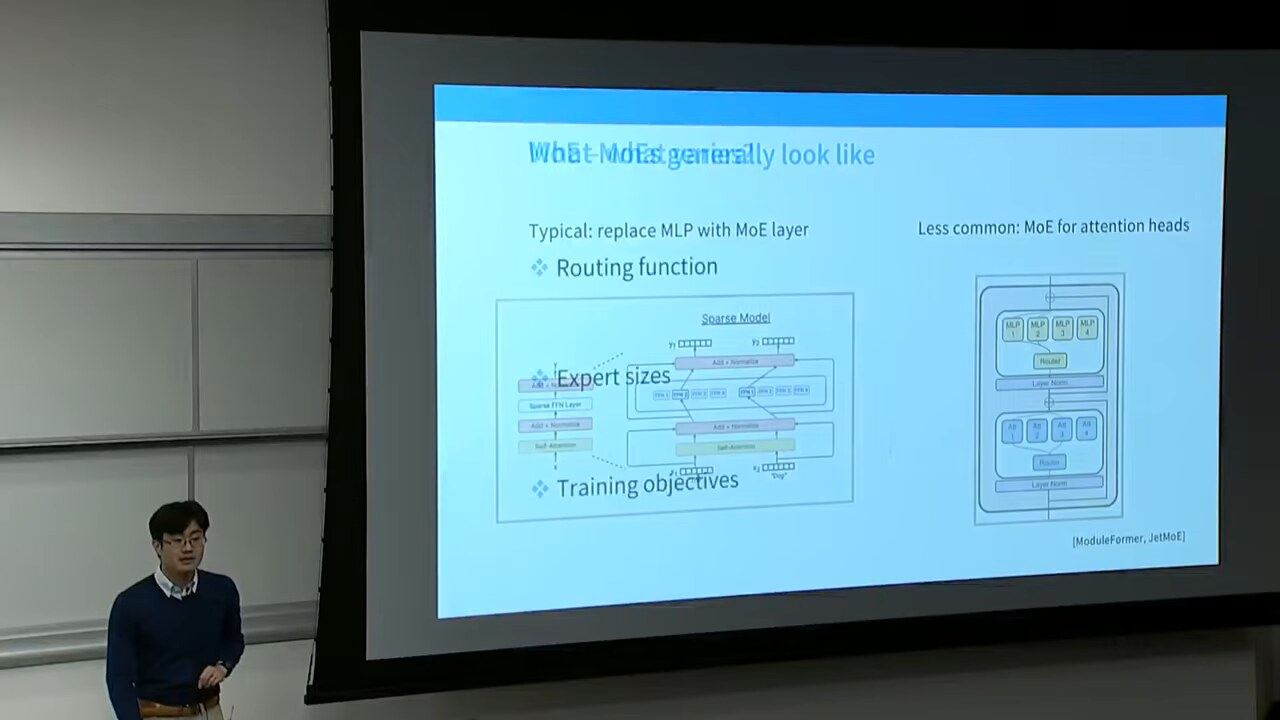
\includegraphics[width=\textwidth]{figures/fig_10_router_attention.jpg}
\caption{Router 与 attention 操作的类比：内积 + softmax，都是在候选集中按相似度加权\protect\footnotemark}
\end{figure}
\footnotetext{视频画面时间区间：00:21:00--00:21:30。}

\begin{knowledgebox}{Router 与 Attention 的对应关系}
\begin{itemize}
\item Attention：query $q$ 与 keys $\{k_j\}$ 内积 $\to$ softmax $\to$ 对 values 加权求和。
\item Router：token 表示 $x$ 与专家向量 $\{e_i\}$ 内积 $\to$ softmax $\to$ 对专家输出加权（并取 top-k 稀疏化）。
\item 二者都可以看作"在候选集中按相似度分配权重"的操作，router 只是额外加了 top-k 截断使其稀疏。
\end{itemize}
\end{knowledgebox}

\subsection{Token-Choice 路由方程}

最常见的路由策略是 \textbf{token-choice（token 选择专家）}：对每个 token，router 计算它对所有专家的偏好分数，取 top-k 个分数最高的专家。

\begin{figure}[H]
\centering
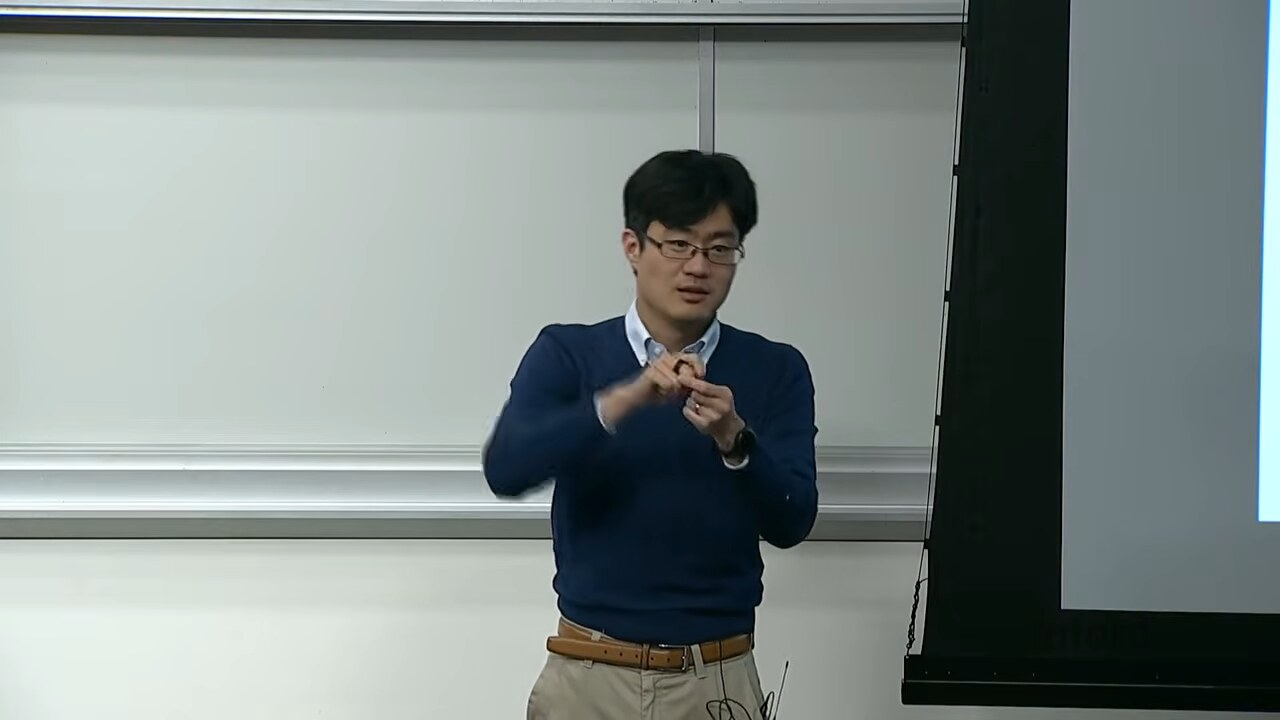
\includegraphics[width=\textwidth]{figures/fig_11_router_equation.jpg}
\caption{Token-choice 路由方程：router 对 token 表示与各专家向量做内积，softmax 后取 top-k，再用归一化后的分数加权\protect\footnotemark}
\end{figure}
\footnotetext{视频画面时间区间：00:19:30--00:20:00。}

形式化地，设 token 表示为 $x\in\mathbb{R}^{d}$，共有 $N$ 个专家，router 维护可学习矩阵 $W\in\mathbb{R}^{N\times d}$（每行 $w_i$ 是专家 $i$ 的"表示向量"）。路由打分为：

\[
g(x) \;=\; \mathrm{softmax}\!\bigl(Wx\bigr) \;=\; \mathrm{softmax}\!\bigl(\langle w_1,x\rangle,\;\ldots,\;\langle w_N,x\rangle\bigr)
\]

然后取分数最高的 $k$ 个专家（top-k），把这些专家的分数重新归一化后作为门控权重 $g_i$，token 的输出为：

\[
y \;=\; \sum_{i\,\in\,\mathrm{top\text{-}k}(g(x))} g_i \cdot \mathrm{FFN}_i(x)
\]

其中只有被选中的 $k$ 个专家参与计算，其余专家不激活——这就是"稀疏"的含义。

\subsubsection{门控权重的两种取法}

关于门控权重 $g_i$ 有两种常见实现。第一种是"先 top-k、再在选中者内重新 softmax 归一化"：

\[
g_i \;=\; \frac{\exp(\langle w_i,x\rangle)}{\sum_{j\in\mathrm{top\text{-}k}} \exp(\langle w_j,x\rangle)}, \qquad i\in\mathrm{top\text{-}k}
\]

第二种是直接保留全局 softmax 中选中专家的原始概率（不再重新归一化），从而保留概率的相对量级。DeepSeek、Mixtral 等多采用前者，使加权系数在同一 token 内可比。

\subsubsection{Expert-Choice 路由：反过来让专家挑 token}

Token-choice 是"token 选专家"。另一种思路 \textbf{expert-choice（专家选 token）}反转方向：每个专家从全 batch 的 token 里挑出它最想处理的固定数量 token。形式上，对专家 $i$，按分数 $\langle w_i, x_t\rangle$ 对所有 token $t$ 排序取前若干：

\[
\mathcal{S}_i \;=\; \mathrm{top\text{-}capacity}\bigl(\{\langle w_i, x_t\rangle : t=1,\ldots,T\}\bigr)
\]

这样负载天然均衡（每个专家都拿满容量），但一个 token 可能被多个专家同时处理或漏掉，破坏了 token 级的因果一致性，因而在自回归生成中不如 token-choice 常用。

\begin{itemize}
\item $x$：当前 token 的隐藏表示。
\item $W$：router 的可学习权重，每行对应一个专家的"原型向量"。
\item $g_i$：token 被分配给专家 $i$ 的门控权重（仅 top-k 非零）。
\item $\mathrm{FFN}_i$：第 $i$ 个专家的前馈子网络。
\item $k$：每个 token 激活的专家数（典型值 1--8）。
\end{itemize}

\begin{figure}[H]
\centering
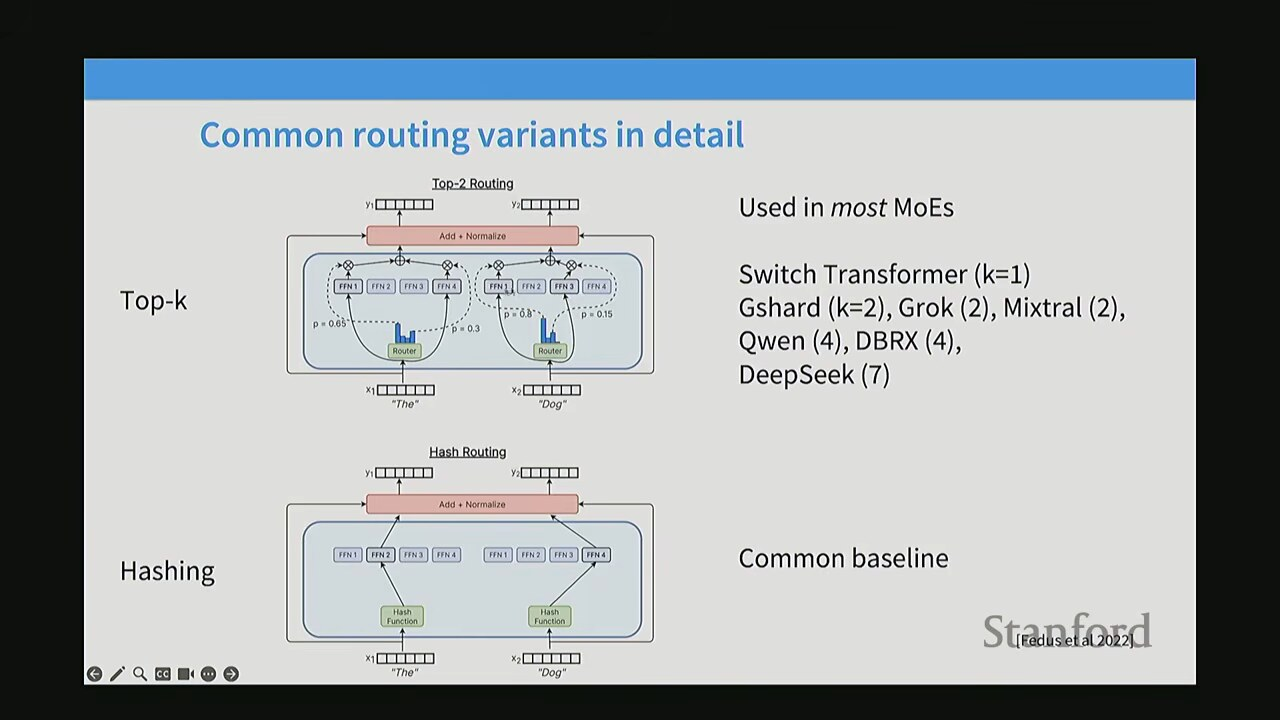
\includegraphics[width=\textwidth]{figures/fig_12_router_weights.jpg}
\caption{Router 权重是否乘到专家输出：不同实现有的只做选择、有的把归一化后的分数作为加权系数\protect\footnotemark}
\end{figure}
\footnotetext{视频画面时间区间：00:21:45--00:22:15。}

\subsection{经典 MoE 模型谱系}

\begin{figure}[H]
\centering
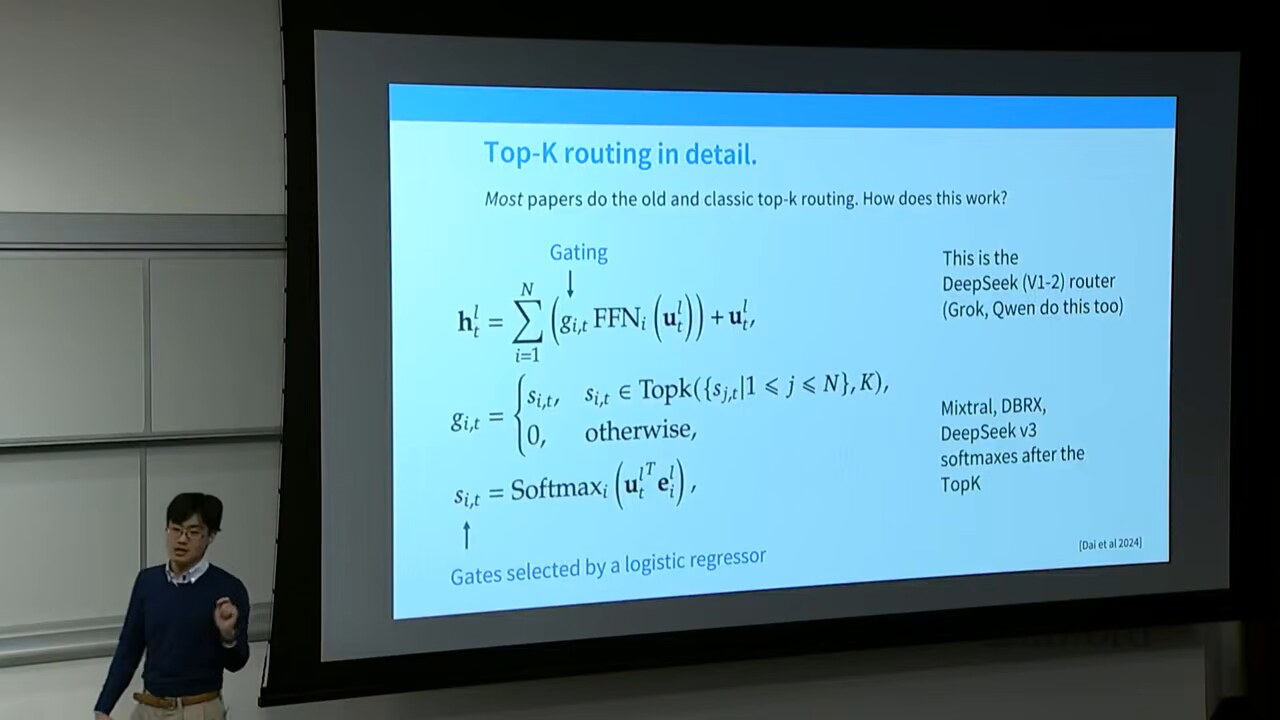
\includegraphics[width=\textwidth]{figures/fig_13_gshard_switch_stmoe.jpg}
\caption{MoE 模型谱系：GShard、Switch Transformer、ST-MoE 等代表性工作的演进\protect\footnotemark}
\end{figure}
\footnotetext{视频画面时间区间：00:31:45--00:32:15。}

\begin{warningbox}{Router 为何如此"简陋"}
有同学提问：router 只是一个线性层加 softmax，参数量很少，为什么不用更复杂的 router？Percy 指出，实践上简单 router 已经足够，而更复杂的 router 反而会增加计算与调参负担，未必带来收益。最优 router 的设计仍是一个开放问题，DeepSeek 的 fine-grained + shared expert 是当前较优的工程答案。
\end{warningbox}

\section{DeepSeek 的核心创新：细粒度专家与共享专家}

\subsection{Fine-grained Expert：把大 FFN 切成更多小专家}

DeepSeek-MoE 的第一个关键想法：与其用少数几个大专家，不如把原本一个大的 FFN 切成更多更小的专家。这样每个专家更"专精"，组合空间更大，路由更灵活，专家专业化（specialization）也更明显。

\begin{figure}[H]
\centering
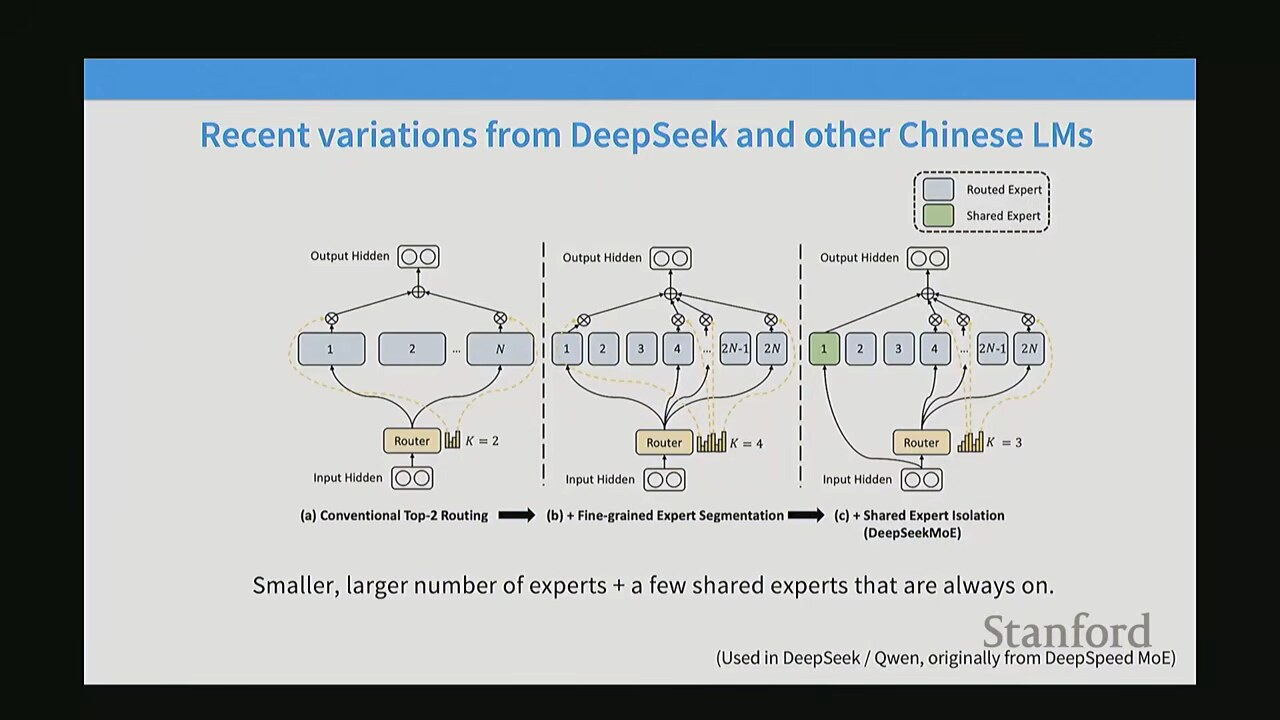
\includegraphics[width=\textwidth]{figures/fig_14_fine_grained_expert.jpg}
\caption{Fine-grained expert：把一个大 FFN 切成多个更小、更专精的专家，扩大组合空间\protect\footnotemark}
\end{figure}
\footnotetext{视频画面时间区间：00:33:00--00:33:30。}

具体地，设 dense FFN 中间层宽度为 $D$。标准 MoE 用 $N$ 个宽度同为 $D$ 的大专家；fine-grained 方案改为 $mN$ 个宽度为 $D/m$ 的小专家，每个 token 仍激活 $mk$ 个（保持总激活宽度 $mk\cdot D/m = kD$ 不变）：

\[
\underbrace{N\text{ 个 } D\text{-宽专家，激活 } k}_{\text{标准 MoE}}
\;\longrightarrow\;
\underbrace{mN\text{ 个 } (D/m)\text{-宽专家，激活 } mk}_{\text{Fine-grained MoE}}
\]

\begin{itemize}
\item 总激活计算量不变（都是 $kD$ 量级），但可选专家数翻 $m$ 倍、组合数从 $\binom{N}{k}$ 涨到 $\binom{mN}{mk}$。
\item 每个专家更窄、更专一，配合 shared expert 后专家分工更清晰。
\end{itemize}

\subsection{Shared Expert：始终激活的通用专家}

\textbf{Shared expert（共享专家）}是 DeepSeek 的第二个核心创新：除了被稀疏路由的 fine-grained expert，还保留一个（或几个）\emph{始终激活}的 shared expert，负责学习所有 token 都需要的通用知识。这样路由专家可以更专注于"差异化"的特征。

\begin{figure}[H]
\centering
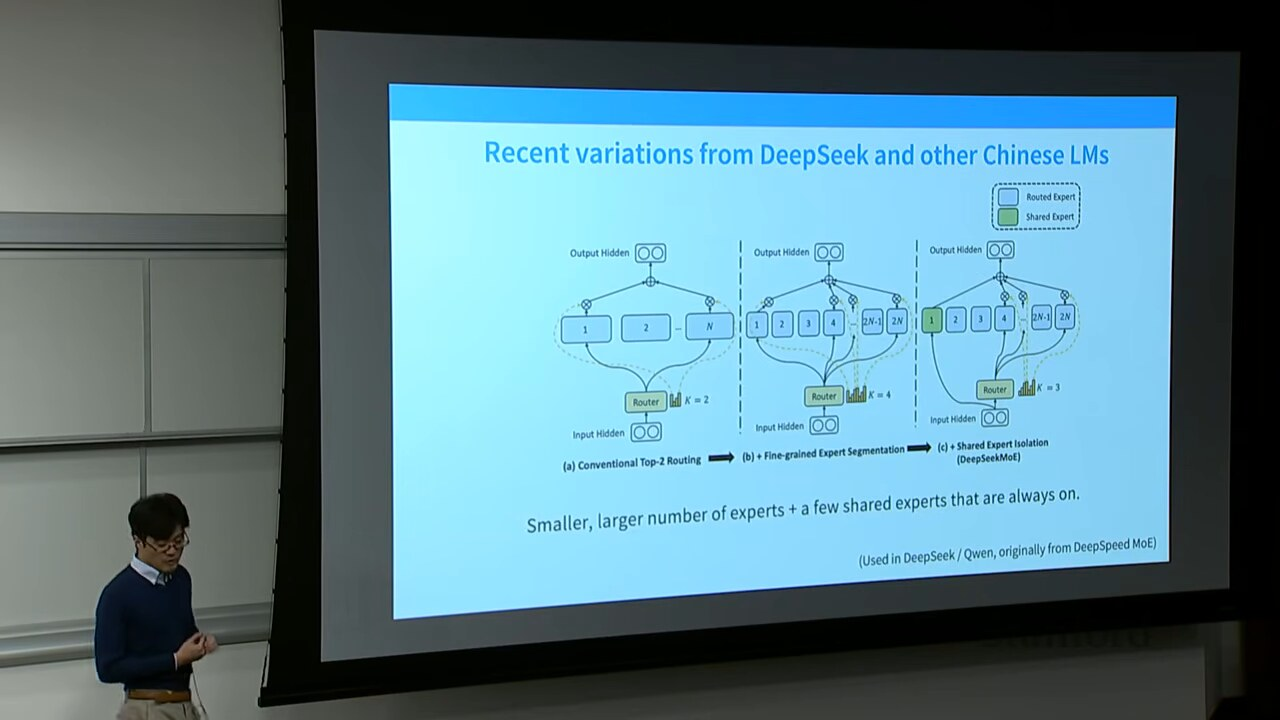
\includegraphics[width=\textwidth]{figures/fig_15_shared_expert.jpg}
\caption{Shared expert：始终激活的共享专家负责通用知识，路由专家则处理差异化特征\protect\footnotemark}
\end{figure}
\footnotetext{视频画面时间区间：00:34:00--00:34:30。}

token 的最终输出因此变为：

\[
y \;=\; \underbrace{\sum_{j} \mathrm{SharedFFN}_j(x)}_{\text{共享专家（恒激活）}} \;+\; \underbrace{\sum_{i\,\in\,\mathrm{top\text{-}k}} g_i \cdot \mathrm{FFN}_i(x)}_{\text{路由专家（稀疏）}}
\]

\begin{itemize}
\item 第一项是若干个 shared expert 的输出之和，对每个 token 都计算，不经过路由。
\item 第二项是 top-k 路由专家的加权输出，与标准 MoE 相同。
\item 这种分工让"通用模式"与"特化模式"解耦，提升专家利用率。
\end{itemize}

\begin{figure}[H]
\centering
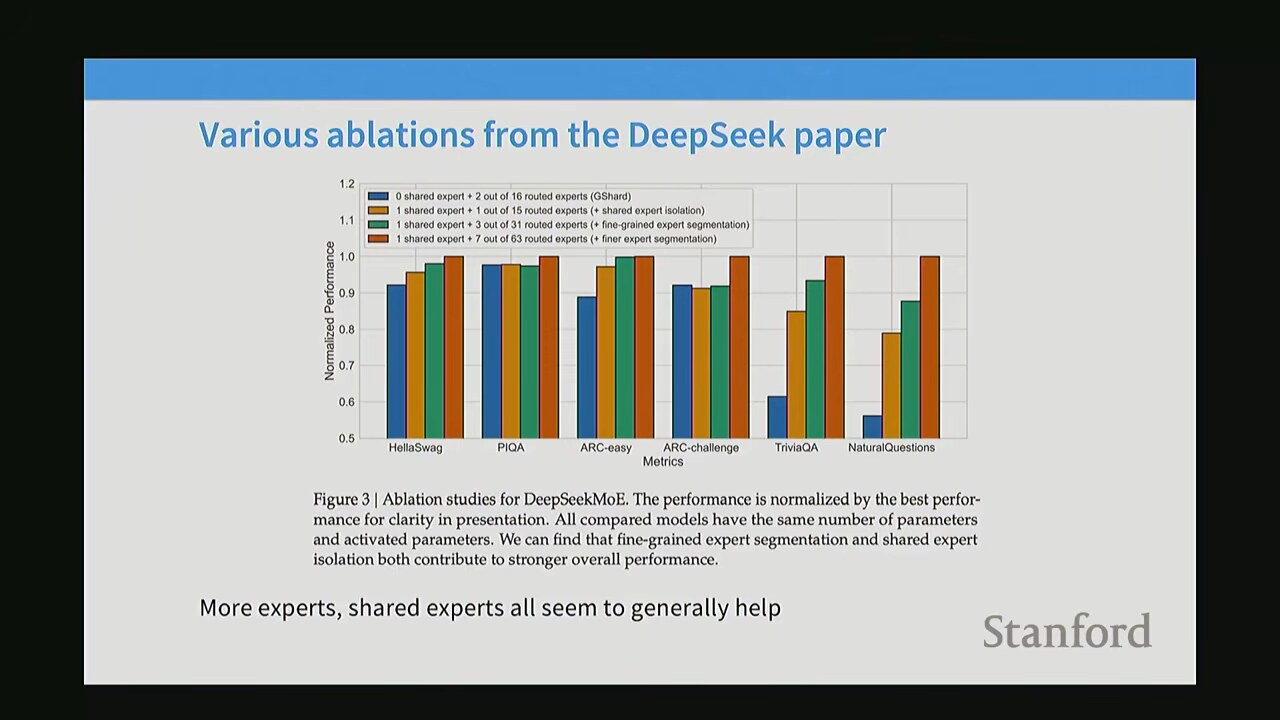
\includegraphics[width=\textwidth]{figures/fig_16_shared_expert_ablation.jpg}
\caption{DeepSeek 关于 shared expert 数量的消融实验：即使只加一个 shared expert，收益也十分明显\protect\footnotemark}
\end{figure}
\footnotetext{视频画面时间区间：00:34:45--00:35:15。}

\begin{importantbox}{DeepSeek 的设计直觉}
Fine-grained + shared expert 的组合可以理解为一种"分工假设"：通用知识（语法、常识）由共享专家承载，避免重复学习；领域/模式特化的知识由众多细粒度路由专家承载，通过路由按需调用。消融实验表明，哪怕只用一个 shared expert，模型性能也有可观提升。
\end{importantbox}

\subsection{参数算术：MoE 与 Dense 的等价}

Percy 做了一组算术来对比：当所有被激活的专家加起来的总宽度等于一个 dense FFN 的宽度时，MoE 每个 token 的计算量与 dense 相当，但可学习的总参数量（全部专家之和）远大于 dense。这正是"同算力下更强"的来源。

\begin{figure}[H]
\centering
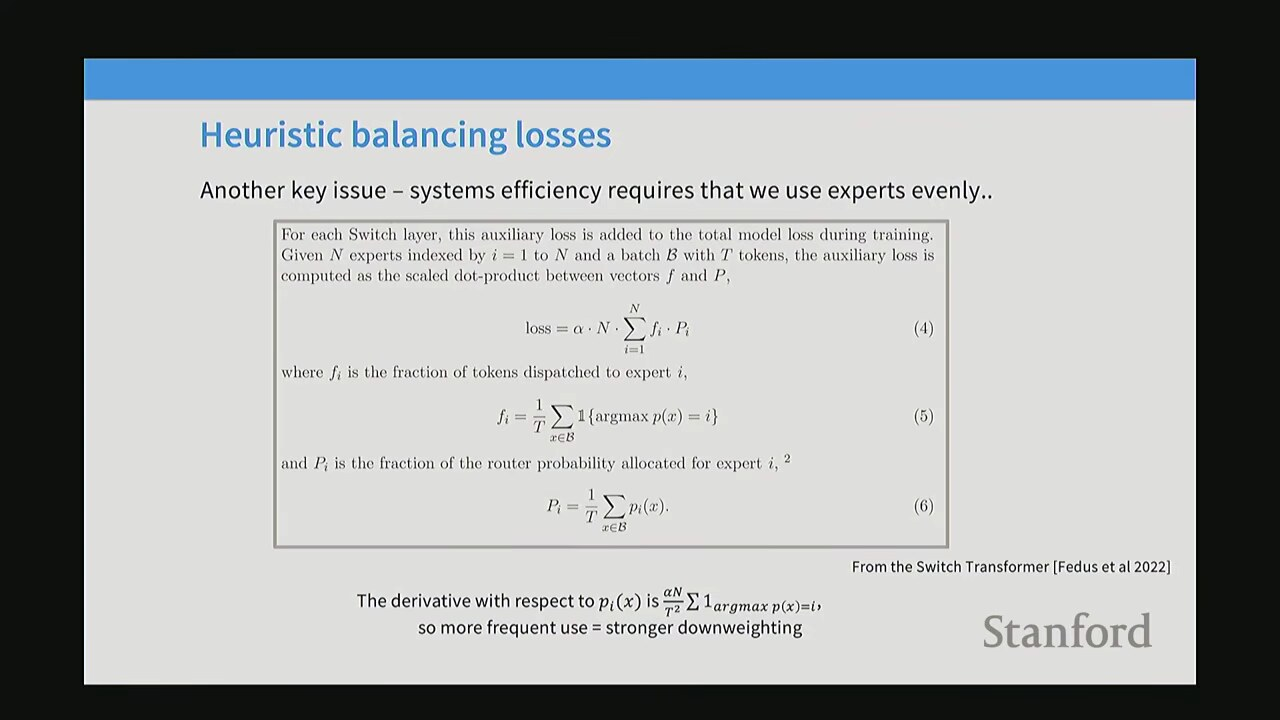
\includegraphics[width=\textwidth]{figures/fig_17_load_balancing_loss.jpg}
\caption{Switch Transformer 的负载均衡损失：以 $f\cdot p$ 内积形式度量专家负载与路由概率的一致性\protect\footnotemark}
\end{figure}
\footnotetext{视频画面时间区间：00:49:30--00:50:00。}

\section{负载均衡：让所有专家都被用上}

\subsection{Routing Collapse：不均衡就会崩溃}

如果不加干预，MoE 训练极易出现 \textbf{routing collapse（路由坍缩）}：router 很快就偏好少数几个专家，绝大多数 token 都涌向它们，其余专家几乎收不到 token 因而得不到训练，模型容量被浪费，性能停滞。

\begin{figure}[H]
\centering
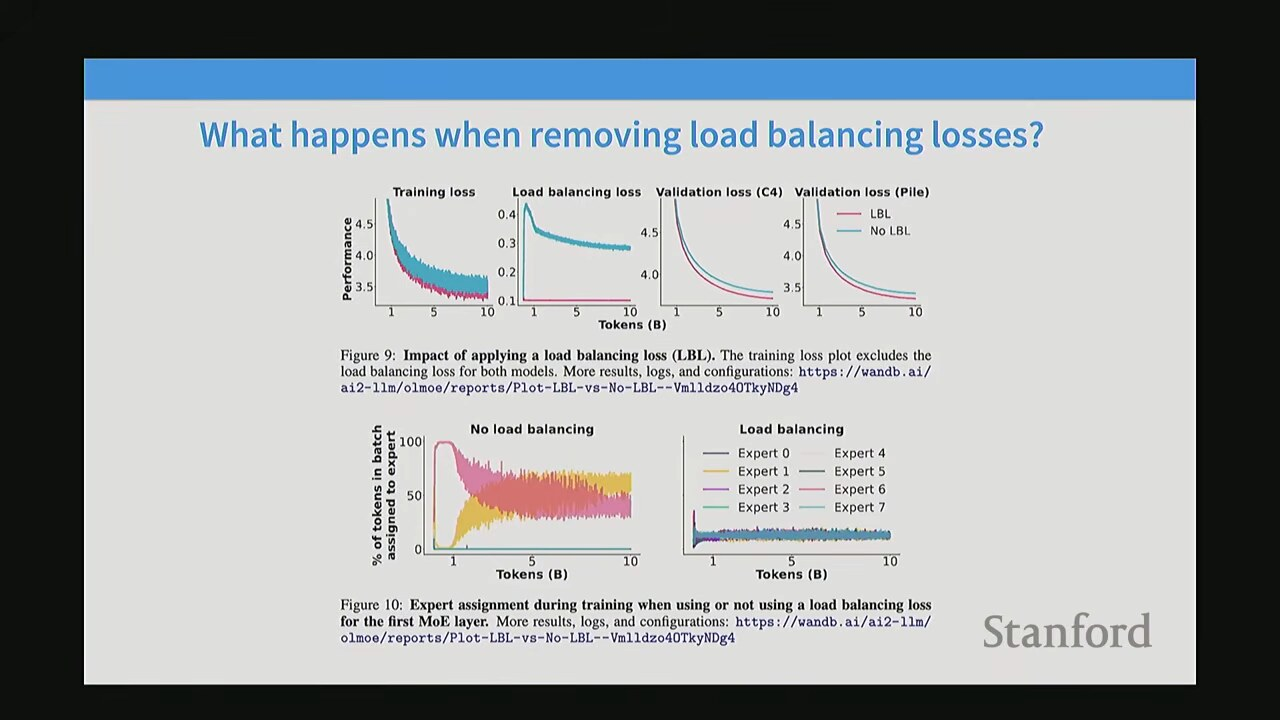
\includegraphics[width=\textwidth]{figures/fig_19_routing_collapse.jpg}
\caption{不做负载均衡时的 routing collapse：少数专家被过度使用，其余专家几乎闲置\protect\footnotemark}
\end{figure}
\footnotetext{视频画面时间区间：00:58:45--00:59:15。}

\begin{warningbox}{Routing Collapse 的恶性循环}
一旦某专家被频繁选中，它的梯度更新更充分、表现更好，router 就更倾向选它——正反馈导致坍缩。最坏情况下 MoE 退化成"只用一两个专家"，相当于白白浪费了其他专家的参数，甚至不如直接训 dense 模型。
\end{warningbox}

\subsection{Switch Transformer 的辅助损失}

Switch Transformer 用一个 \textbf{辅助损失（auxiliary loss）}强制专家负载均匀。设一个 batch 内：

\[
f_i \;=\; \frac{\text{被路由到专家 } i \text{ 的 token 数}}{\text{batch 内总 token 数}}, \qquad p_i \;=\; \frac{1}{T}\sum_{t=1}^{T} \mathrm{softmax}(Wx_t)_i
\]

\begin{itemize}
\item $f_i$：专家 $i$ 实际接收的 token 比例（fraction of tokens dispatched）。
\item $p_i$：router 给专家 $i$ 的平均概率（average router probability）。
\item $T$：batch 内 token 总数。
\end{itemize}

负载均衡损失定义为二者的内积：

\[
\mathcal{L}_{\text{balance}} \;=\; N \cdot \sum_{i=1}^{N} f_i \, p_i
\]

当所有专家负载完全均匀时 $f_i=p_i=1/N$，此时该损失取最小值 $N\cdot N\cdot(1/N)^2 = 1$；负载越不均，损失越大。把它以一个小权重加到主训练损失上，就能推动 router 把 token 均匀分配。

可以验证：若只有一个专家垄断（$f_1=p_1=1$，其余为 0），则

\[
\mathcal{L}_{\text{balance}}^{\text{worst}} \;=\; N\cdot(1\cdot 1) \;=\; N \;\gg\; 1
\]

最坏情形的损失是均衡情形的 $N$ 倍，梯度方向明确地把概率从过载专家推向欠载专家，从而抑制坍缩。

\subsection{DeepSeek V3：Auxiliary-Loss-Free Balancing}

辅助损失有效，但它会扭曲主损失的梯度、引入超参（权重）、且容易和主目标冲突。DeepSeek V3 提出了 \textbf{auxiliary-loss-free balancing（无辅助损失的均衡）}：为每个专家维护一个可学习的偏置 $b_i$，把它加到 router 的 logits 上影响路由选择，但\emph{不}参与最终门控权重的计算，也不产生额外损失。

\begin{figure}[H]
\centering
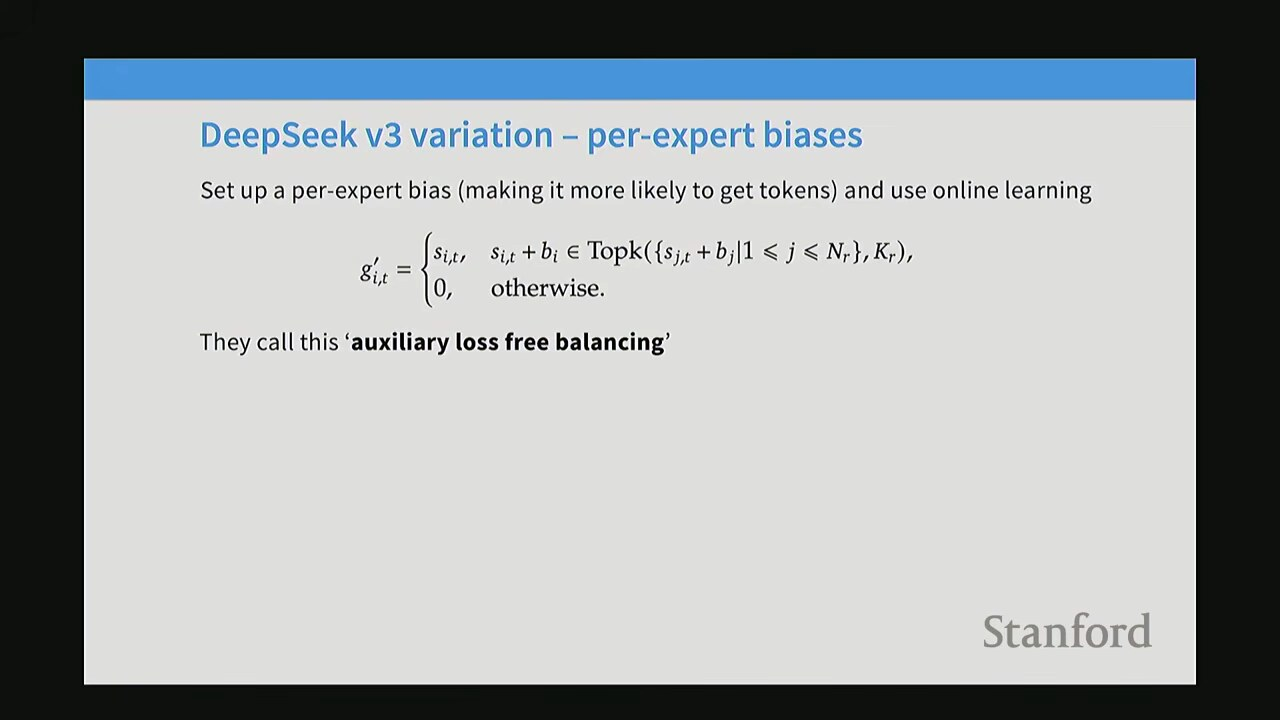
\includegraphics[width=\textwidth]{figures/fig_18_aux_loss_free.jpg}
\caption{DeepSeek V3 的 auxiliary-loss-free balancing：用可学习偏置 $b_i$ 调节路由，不引入辅助损失\protect\footnotemark}
\end{figure}
\footnotetext{视频画面时间区间：00:53:45--00:54:15。}

形式上，路由打分变为：

\[
s_i(x) \;=\; \langle w_i,\, x\rangle \;+\; b_i, \qquad \text{选择 top-k 依据 } s_i,\ \text{但门控权重 } g_i \text{ 仍由不含 } b_i \text{ 的 softmax 决定}
\]

\begin{itemize}
\item $b_i$：每个专家一个可学习标量，由一个简单规则更新——若专家 $i$ 负载偏低就上调 $b_i$，偏高就下调。
\item 这样均衡是"通过调整选择倾向"实现的，而非通过损失项扭曲梯度，对主任务更友好。
\end{itemize}

DeepSeek 的偏置更新遵循一个轻量级的符号规则（不通过反向传播，而是按统计量直接调整）：

\[
b_i \;\leftarrow\; b_i \;+\; \eta_{b}\cdot\mathrm{sign}\!\bigl(\bar{f}^{\text{target}} - f_i\bigr)
\]

\begin{itemize}
\item $f_i$：当前步专家 $i$ 实际接收的 token 比例。
\item $\bar{f}^{\text{target}}=1/N$：理想均匀负载下的目标比例。
\item $\eta_b$：偏置更新的步长（通常很小，如 $10^{-3}$）。
\item 当 $f_i < 1/N$（专家 $i$ 欠载），符号为正，$b_i$ 增大，使该专家更容易被选中；反之则减小。
\end{itemize}

\begin{knowledgebox}{为何"无损失"更优雅}
辅助损失需要调权重：太轻压不住坍缩，太重损害主任务。偏置法把均衡与主梯度解耦，更新规则直接、可解释，且不会污染语言建模的梯度信号。DeepSeek 仍保留了一个很小的 complementary sequence-wise auxiliary loss 作为补充，但主负荷已由 bias 承担。
\end{knowledgebox}

\section{MoE 的训练工程难题}

\subsection{Expert Parallelism 与 All-to-All 通信}

把不同专家放到不同设备后，每个 token 可能要发给远端设备上的专家处理，算完再取回。这需要一次 \textbf{all-to-all} 集体通信：每个设备把"属于别的设备专家"的 token 发出去，并接收"属于自己专家"的 token。

\begin{figure}[H]
\centering
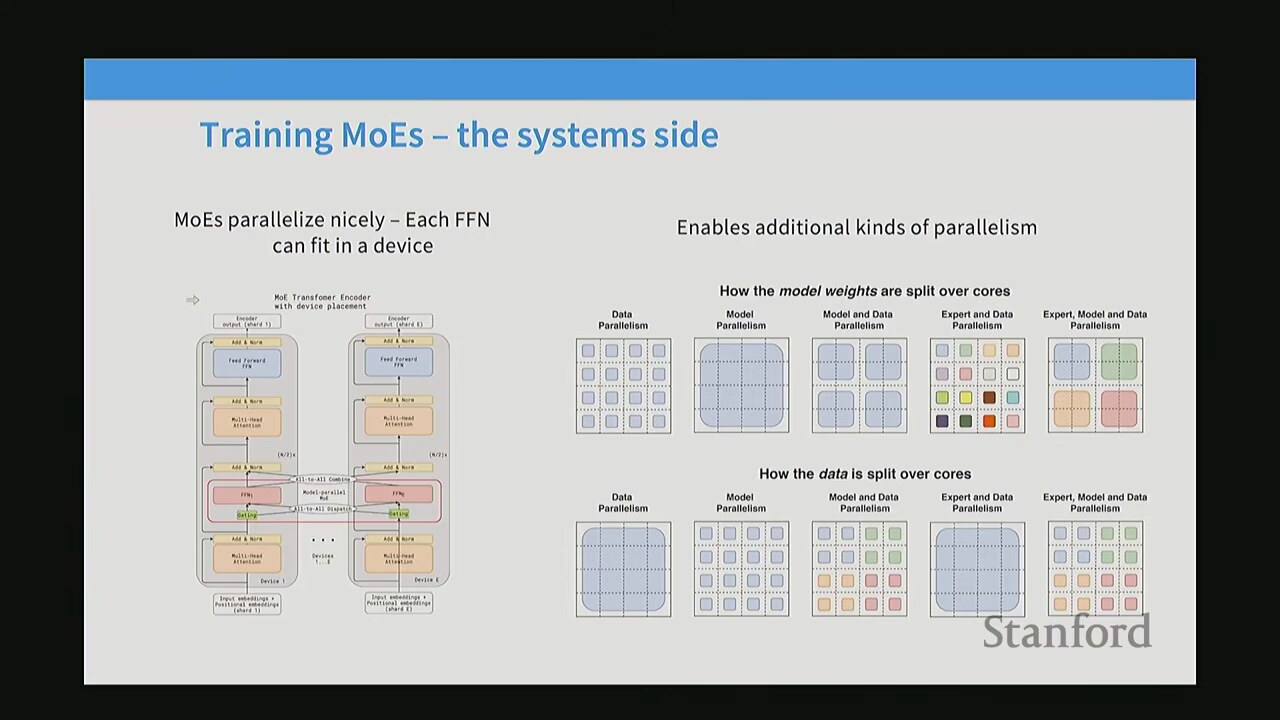
\includegraphics[width=\textwidth]{figures/fig_20_expert_parallel_arch.jpg}
\caption{专家并行架构：router 选定专家后，通过 all-to-all dispatch 把 token 送到对应设备，计算后再 all-to-all 回传\protect\footnotemark}
\end{figure}
\footnotetext{视频画面时间区间：00:59:45--01:00:15。}

\begin{warningbox}{通信成本不可忽视}
在数据中心内，跨设备带宽远低于设备内显存带宽。all-to-all 的通信量随专家数和 token 数增长。若不加以控制，通信会成为 MoE 训练的主要瓶颈，甚至抵消稀疏化带来的算力节省。因此 DeepSeek 引入了专门的通信均衡损失。
\end{warningbox}

单步 all-to-all 的通信量大致正比于被路由的 token 总量。设每个 token 表示维度为 $d$、batch 内 token 数为 $T$、平均每个 token 激活 $k$ 个专家，且采用 $D$ 路专家并行，则 dispatch 与 combine 两阶段的通信量约为：

\[
\text{Comm} \;\approx\; 2 \cdot T \cdot k \cdot d \cdot \beta
\]

\begin{itemize}
\item 系数 2 来自 dispatch（发送）与 combine（回收）两个方向。
\item $\beta$ 为跨设备带宽利用率因子。
\item 当 $T$、$k$、$d$ 都很大时，通信量与专家计算量同量级，必须用均衡损失与 top-M 设备路由压缩。
\end{itemize}

\subsection{Token Dropping：容量溢出时丢弃}

为保证负载可预测，每个专家被分配一个 \textbf{容量（capacity）}：一个固定大小的缓冲区，只能容纳一定数量的 token。当路由到某专家的 token 超过容量时，\emph{多余的 token 被丢弃}（token dropping），通常直接走残差通路（相当于跳过这一层 FFN）。

\begin{figure}[H]
\centering
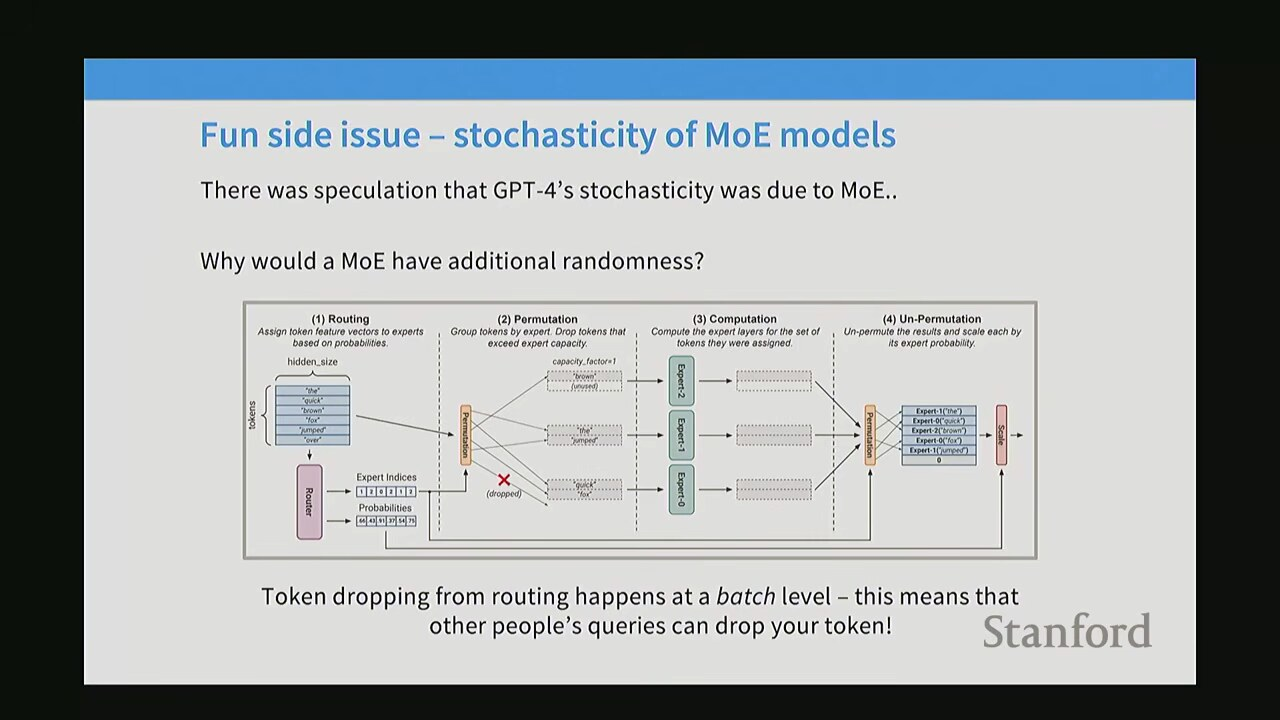
\includegraphics[width=\textwidth]{figures/fig_21_token_dropping.jpg}
\caption{Token dropping：专家容量溢出时丢弃多余 token，被丢弃的 token 走残差通路\protect\footnotemark}
\end{figure}
\footnotetext{视频画面时间区间：01:03:45--01:04:15。}

容量由一个 \textbf{capacity factor（容量因子）}控制：

\[
\text{capacity} \;=\; \text{capacity\_factor} \;\times\; \frac{T}{N}
\]

\begin{itemize}
\item $T$：batch 内 token 总数。
\item $N$：专家数。
\item $T/N$：理想均匀负载下每个专家应得的 token 数。
\item capacity\_factor：略大于 1（如 1.25），既留出余量应对不均，又限制最大计算量以保证调度可预测。
\end{itemize}

\begin{practicebox}{工程权衡}
容量因子是一个典型的权衡旋钮：调大 → 训练稳定、几乎不丢 token，但计算与显存开销上升；调小 → 开销下降，但丢弃率升高、可能损害性能。实践中常在 1.0--1.5 之间，并配合负载均衡损失把丢弃率压到很低。
\end{practicebox}

\subsection{Z-Loss：稳定 Router 的 Softmax}

Router 的 softmax 对极端 logit 值很敏感：若某个 logit 过大，softmax 会饱和、梯度消失或爆炸，引发训练不稳定。\textbf{Z-loss} 对 router logits 的平方和（或类似形式）施加一个小的正则，把 logits 拉回合理范围，从而稳定训练。

\begin{figure}[H]
\centering
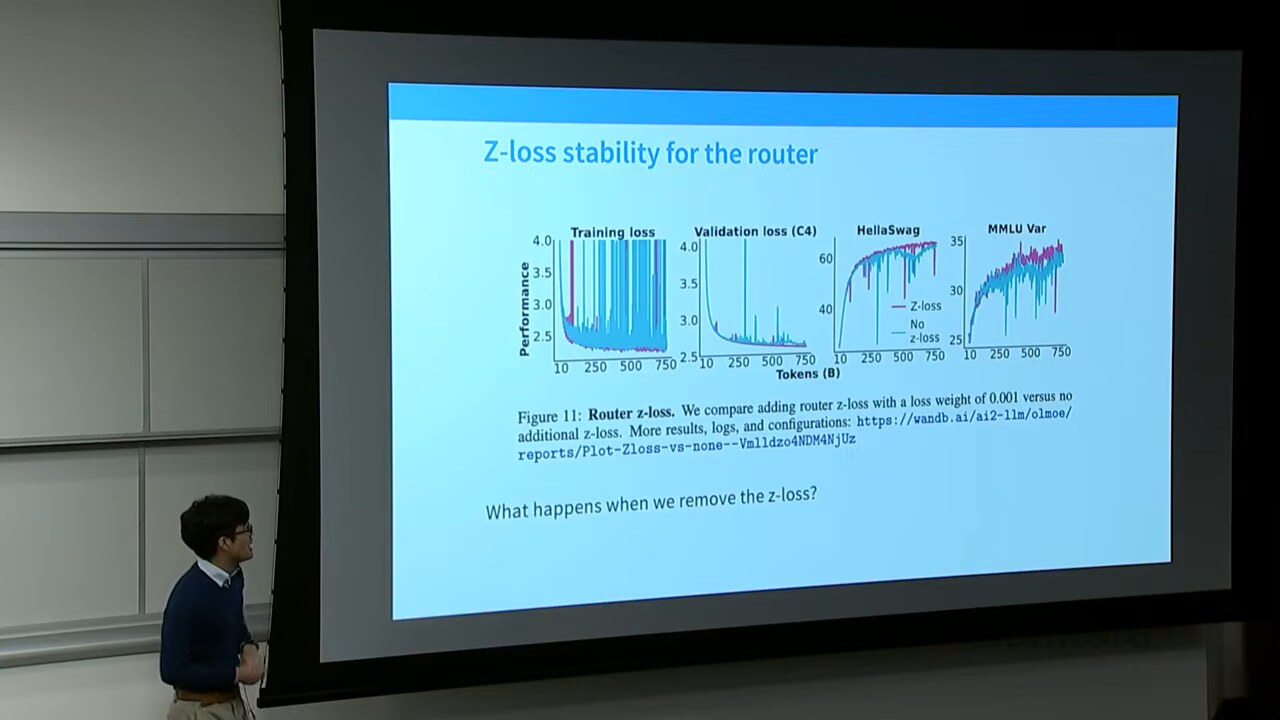
\includegraphics[width=\textwidth]{figures/fig_22_z_loss.jpg}
\caption{Z-loss 正则：对 router 的 softmax logits 加约束，显著缩小有无正则时的训练稳定性差距\protect\footnotemark}
\end{figure}
\footnotetext{视频画面时间区间：01:06:30--01:07:00。}

设 router logits 为 $z = (z_1,\ldots,z_N)$，z-loss 形如：

\[
\mathcal{L}_{z} \;=\; \frac{1}{N}\sum_{i=1}^{N} z_i^{2}
\]

以小权重加入总损失。其作用是抑制 logital 幅度过大，避免 softmax 进入数值不稳定区域。Percy 展示的对比显示，有 z-loss 与无 z-loss 之间存在"相当明显的差距（pretty noticeable gap）"——这是 MoE 训练稳定性最划算的"保险丝"之一。

为什么平方惩罚能稳定训练？考虑 softmax 概率 $p_i = \exp(z_i)/\sum_j\exp(z_j)$ 对 logit $z_i$ 的梯度：

\[
\frac{\partial p_i}{\partial z_i} \;=\; p_i(1-p_i)
\]

当某个 $z_i$ 过大时 $p_i\to 1$，梯度趋于零，路由完全锁死、无法纠正。z-loss 把 $z_i$ 拉回 0 附近，使 $p_i$ 保持适中、梯度健康，路由器才能持续学习。

\begin{importantbox}{MoE 训练稳定性的三道保险}
\begin{itemize}
\item \textbf{负载均衡损失 / bias 均衡}：防止 routing collapse，保证所有专家被利用。
\item \textbf{Z-loss}：稳定 router 的 softmax，防止 logit 爆炸。
\item \textbf{Router 用 float32 计算}：路由打分这一步用更高精度，避免低精度下的路由抖动。三者叠加，才能让大规模 MoE 稳定收敛。
\end{itemize}
\end{importantbox}

\section{DeepSeek V2 与 V3：把 MoE 推到极致}

\subsection{规模演进：16B → 236B → 671B}

DeepSeek 系列展示了 MoE 路线的规模演进：V1 约 16B 总参 / 2.8B 激活；V2 约 236B 总参 / 21B 激活；V3 约 671B 总参 / 37B 激活。激活参数（决定每个 token 计算量）远小于总参数，使得超大模型也能以可控成本训练和推理。

\begin{figure}[H]
\centering
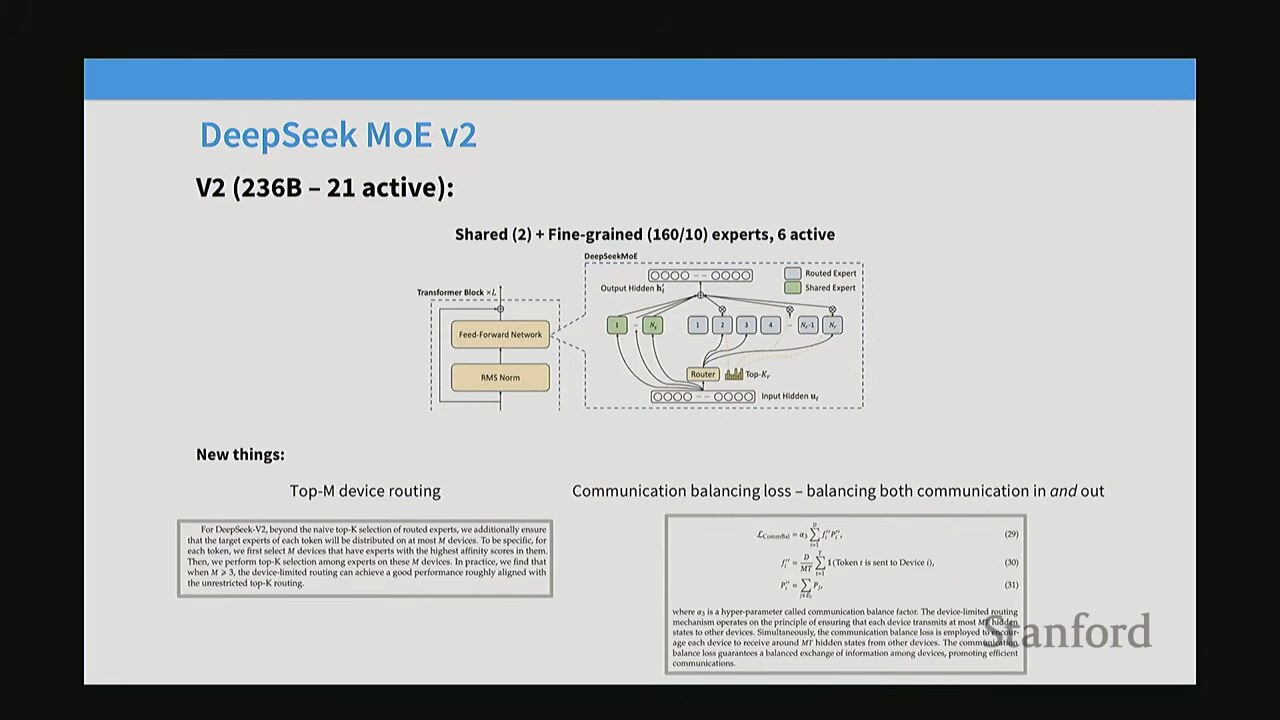
\includegraphics[width=\textwidth]{figures/fig_23_v2_236b.jpg}
\caption{DeepSeek V2：约 236B 总参数、21B 激活参数，是 fine-grained + shared expert 的代表\protect\footnotemark}
\end{figure}
\footnotetext{视频画面时间区间：01:11:45--01:12:15。}

\begin{figure}[H]
\centering
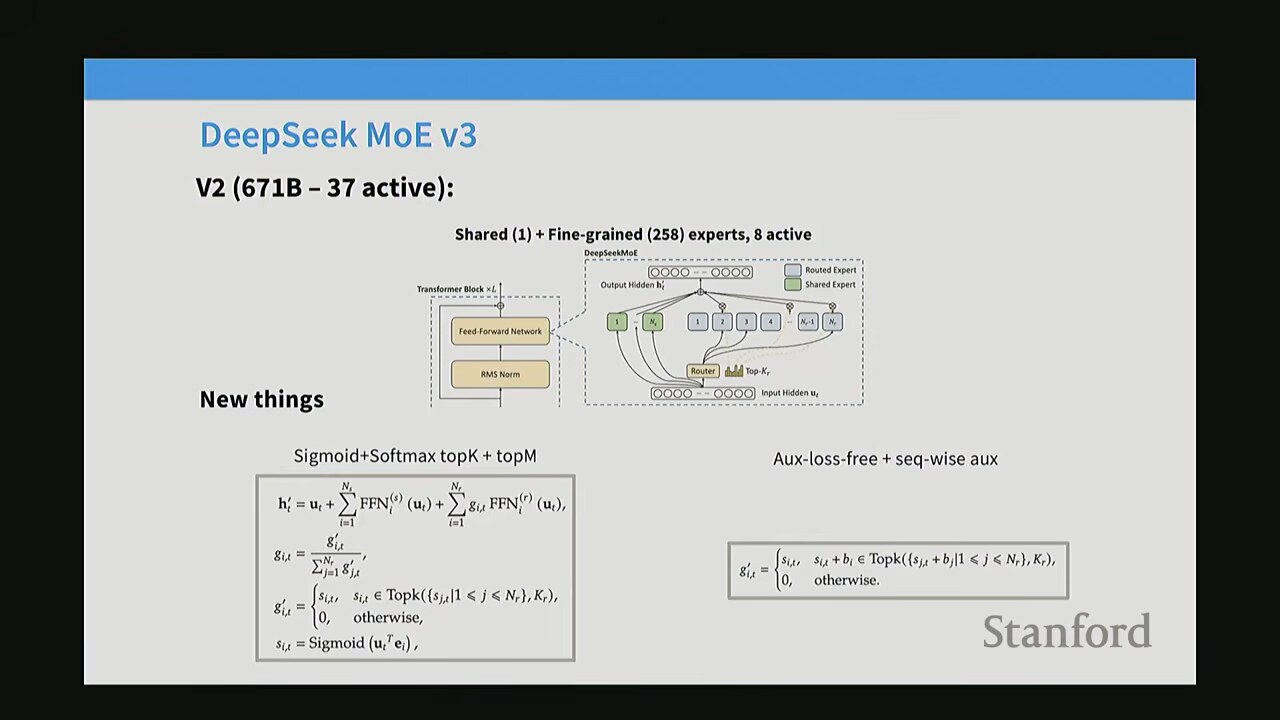
\includegraphics[width=\textwidth]{figures/fig_25_v3_671b.jpg}
\caption{DeepSeek V3：约 671B 总参数、37B 激活参数，在 V2 基础上进一步扩大规模\protect\footnotemark}
\end{figure}
\footnotetext{视频画面时间区间：01:14:15--01:14:45。}

\subsection{通信开销与均衡损失}

当专家数和设备数都很大时，all-to-all 通信成本会急剧上升。DeepSeek 同时考虑 \textbf{input communication cost}（dispatch）和 \textbf{output communication cost}（combine），并引入专门的 \textbf{communication balancing loss} 让通信负载也均匀分布。

\begin{figure}[H]
\centering
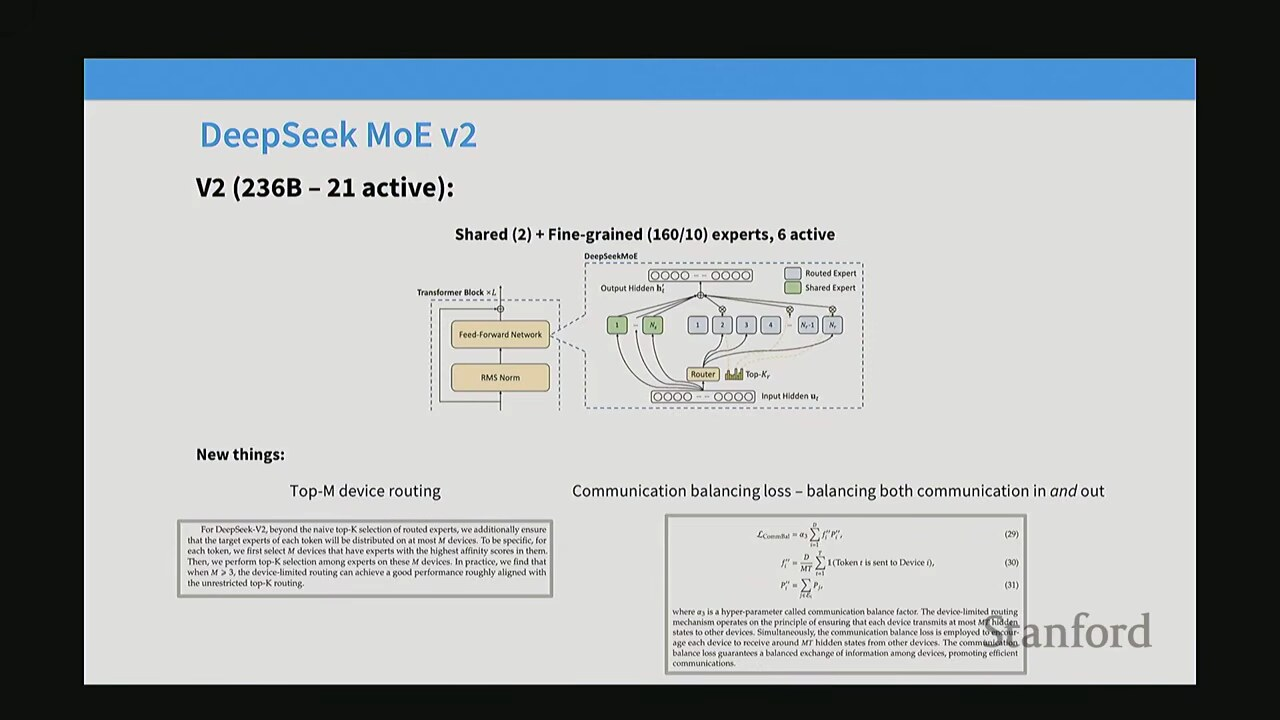
\includegraphics[width=\textwidth]{figures/fig_24_communication_cost.jpg}
\caption{专家并行的通信开销：需同时权衡 dispatch（输入）与 combine（输出）两个方向的通信\protect\footnotemark}
\end{figure}
\footnotetext{视频画面时间区间：01:13:30--01:14:00。}

\begin{figure}[H]
\centering
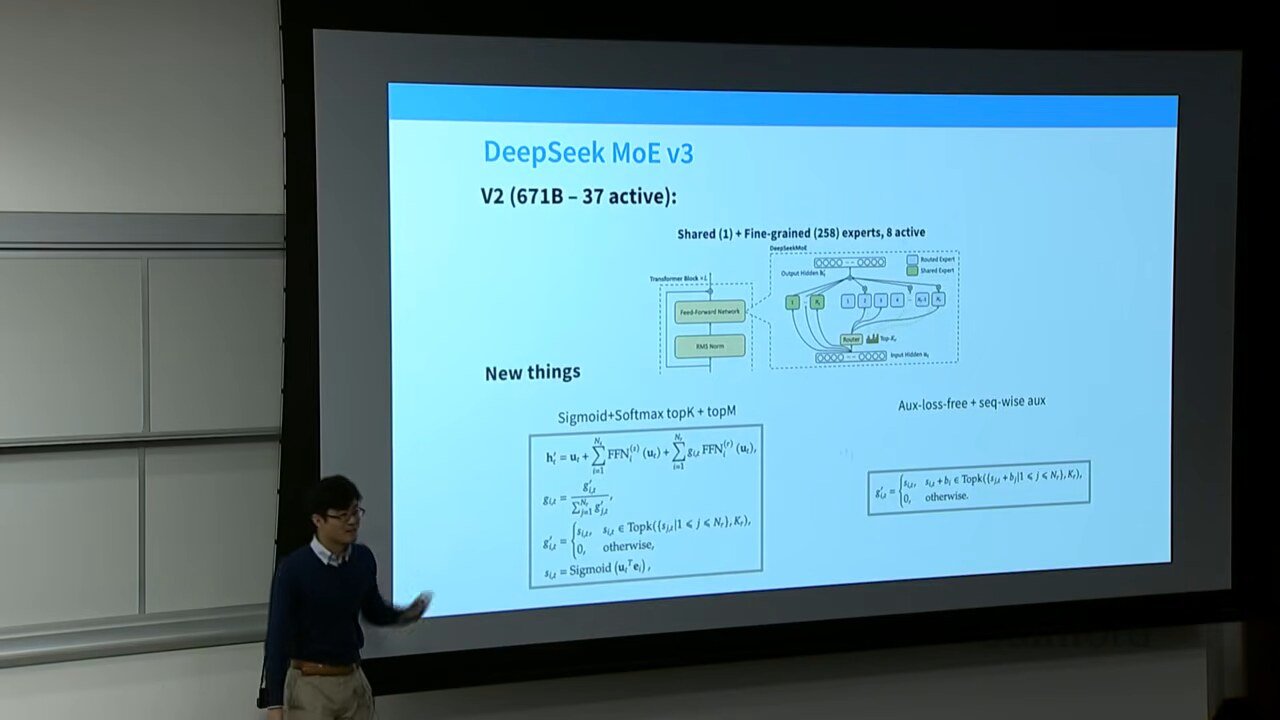
\includegraphics[width=\textwidth]{figures/fig_26_comm_loss.jpg}
\caption{通信均衡损失：让各设备的 input/output 通信量也趋于均衡\protect\footnotemark}
\end{figure}
\footnotetext{视频画面时间区间：01:16:15--01:16:45。}

\subsection{Top-M Device Routing：限制通信范围}

为控制通信成本，DeepSeek 还采用 \textbf{Top-M device routing}：先在"设备"层面做 top-M 选择（把 token 限制在 M 个设备内），再在这 M 个设备的专家中做 top-K 路由。这样通信只发生在少数设备之间，避免了全局 all-to-all 的开销。

\begin{knowledgebox}{两级路由的逻辑}
全局 all-to-all（所有设备两两通信）在大规模下非常昂贵。两级路由——先 top-M 设备、再 top-K 专家——把通信范围从"全部设备"收缩到"M 个设备"，在保持专家多样性的同时大幅降低通信量。这是 MoE 工程化中"用少量选择精度换大量通信节省"的典型设计。
\end{knowledgebox}

\section{DeepSeek 的注意力与预测创新：MLA 与 MTP}

\subsection{MLA：Multi-head Latent Attention 压缩 KV Cache}

MoE 解决了 FFN 的稀疏化，但长上下文下 attention 的 \textbf{KV cache}（存放历史 token 的 key/value）会占用巨量显存。DeepSeek V2 提出 \textbf{MLA（Multi-head Latent Attention）}：用一个低维的 \emph{latent vector}（隐向量）压缩 KV cache，推理时再上投影回完整的 K/V。

\begin{figure}[H]
\centering
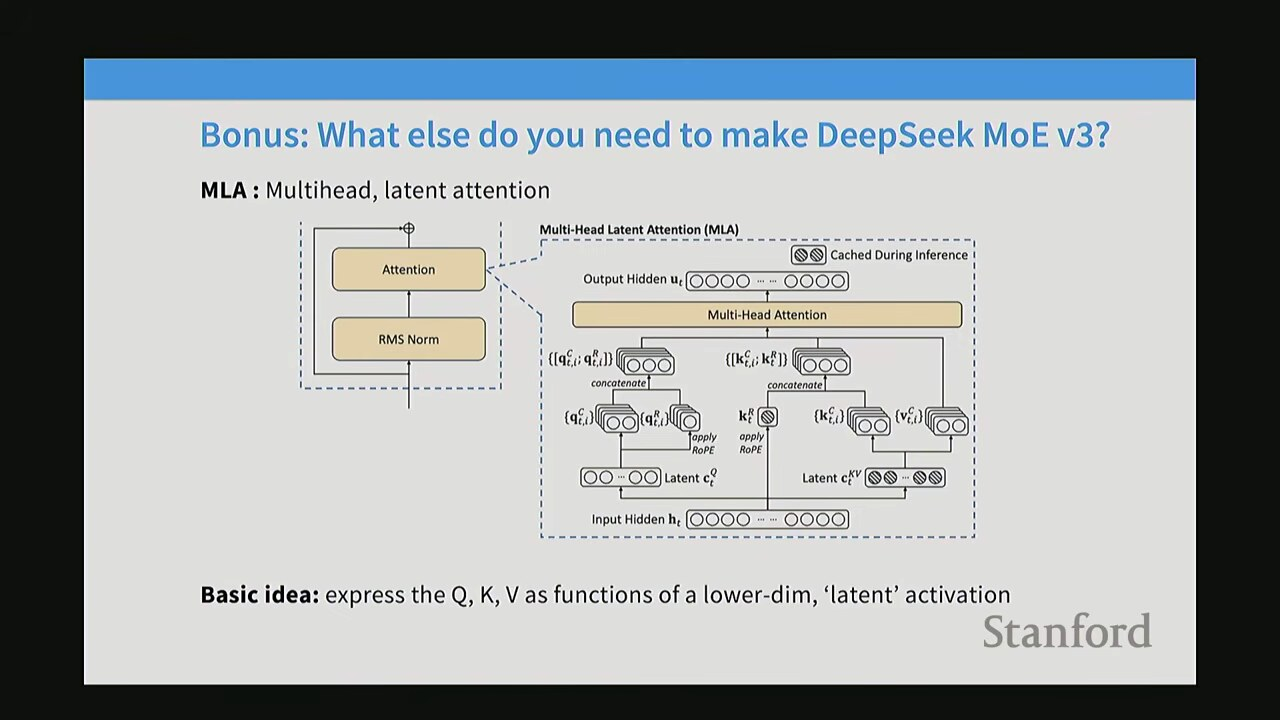
\includegraphics[width=\textwidth]{figures/fig_27_mla.jpg}
\caption{MLA（Multi-head Latent Attention）：通过低维隐向量压缩 KV cache，推理时上投影还原\protect\footnotemark}
\end{figure}
\footnotetext{视频画面时间区间：01:17:00--01:17:30。}

核心机制可表述为：把 token 的隐藏表示 $h$ 先 \emph{下投影}成低维隐向量 $c$：

\[
c \;=\; W_{\text{down}}\, h, \qquad c\in\mathbb{R}^{d_c},\ \ d_c \ll d
\]

KV cache 里只存 $c$（维度小、显存省）。需要 K/V 时，再用 \emph{上投影} 矩阵把它投影回多头所需的 K、V：

\[
K \;=\; W_{K}^{\text{up}}\, c, \qquad V \;=\; W_{V}^{\text{up}}\, c
\]

\begin{figure}[H]
\centering
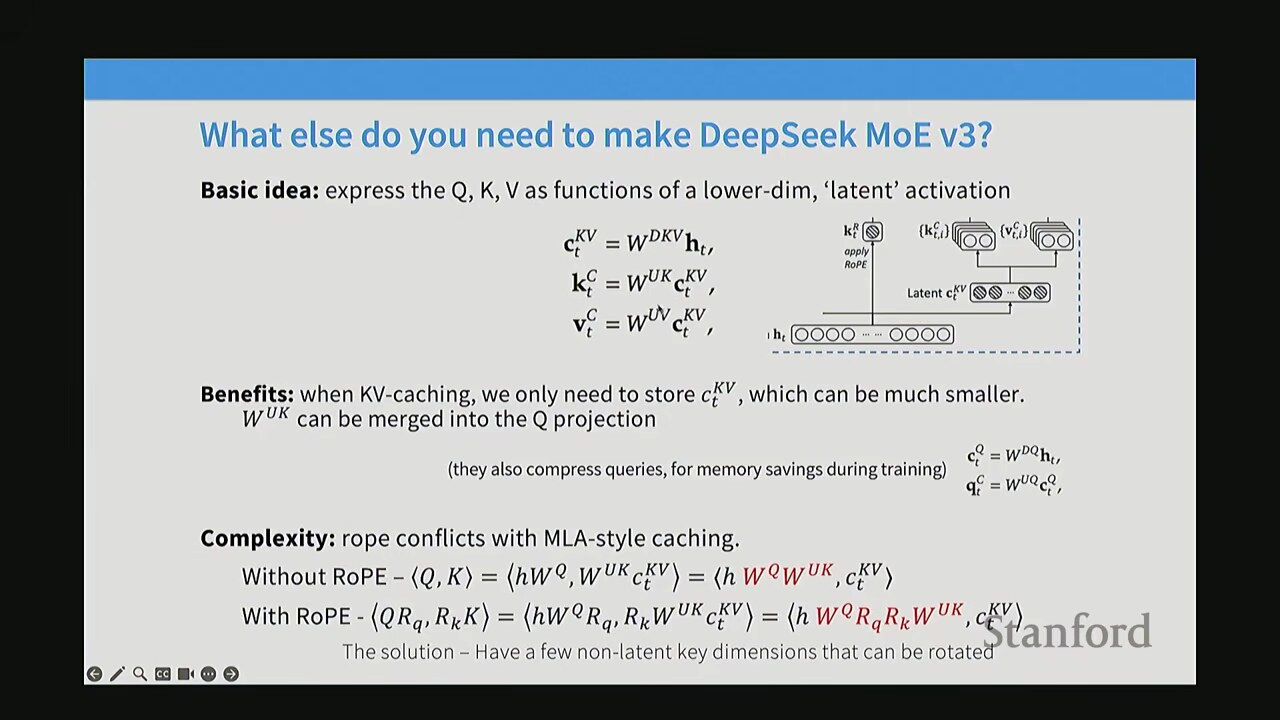
\includegraphics[width=\textwidth]{figures/fig_28_mla_kv_compress.jpg}
\caption{MLA 的 KV cache 压缩：只缓存低维隐向量，Q 也经投影，注意力在不压缩维度上计算\protect\footnotemark}
\end{figure}
\footnotetext{视频画面时间区间：01:18:15--01:18:45。}

\begin{itemize}
\item $h$：token 的原始隐藏表示（高维）。
\item $c$：压缩后的低维隐向量（KV cache 实际存储的对象）。
\item $W_{\text{down}},W_{K}^{\text{up}},W_{V}^{\text{up}}$：下投影与上投影矩阵。
\item 由于只缓存 $c$，长上下文推理的显存占用大幅下降。
\end{itemize}

对于多头注意力中的第 $m$ 个头，注意力权重与输出按标准方式计算：

\[
\mathrm{Att}_m(Q_m, K_m, V_m) \;=\; \mathrm{softmax}\!\left(\frac{Q_m K_m^{\top}}{\sqrt{d_m}}\right) V_m
\]

其中 $Q_m = W_m^Q\, c_q$、$K_m = W_m^{K,\text{up}}\, c$、$V_m = W_m^{V,\text{up}}\, c$ 都由（压缩后的）隐向量上投影得到。注意查询侧 $Q$ 同样经由一个下投影—上投影的两段式结构，使 Q 与 K/V 在压缩潜空间里完成关联。缓存里只存低维 $c$，推理时再展开为各头的 K/V，从而在多头维度上"展开"而不"存储"，显存随 $d_c$（而非完整多头维度）增长。

\begin{importantbox}{MLA 的关键收益}
长上下文推理中，KV cache 显存往往是主要瓶颈。MLA 把缓存维度从 $d$ 压到 $d_c\ll d$，在几乎不损失质量的前提下显著降低显存，使得 DeepSeek V3 能支持更长的上下文窗口。其代价是上投影引入的额外计算，但在推理时这笔计算远小于省下的显存访问成本。
\end{importantbox}

\subsection{MTP：Multi-Token Prediction 预测下一个}

标准语言模型一次预测一个 token。DeepSeek V3 还加入了 \textbf{MTP（Multi-Token Prediction）}：一个轻量级的额外预测头，在主头预测第 $t+1$ 个 token 的同时，预测第 $t+2$ 个 token。训练时这提供了额外的监督信号（让模型"多想一步"），推理时这个额外头可用于投机解码加速。

\begin{figure}[H]
\centering
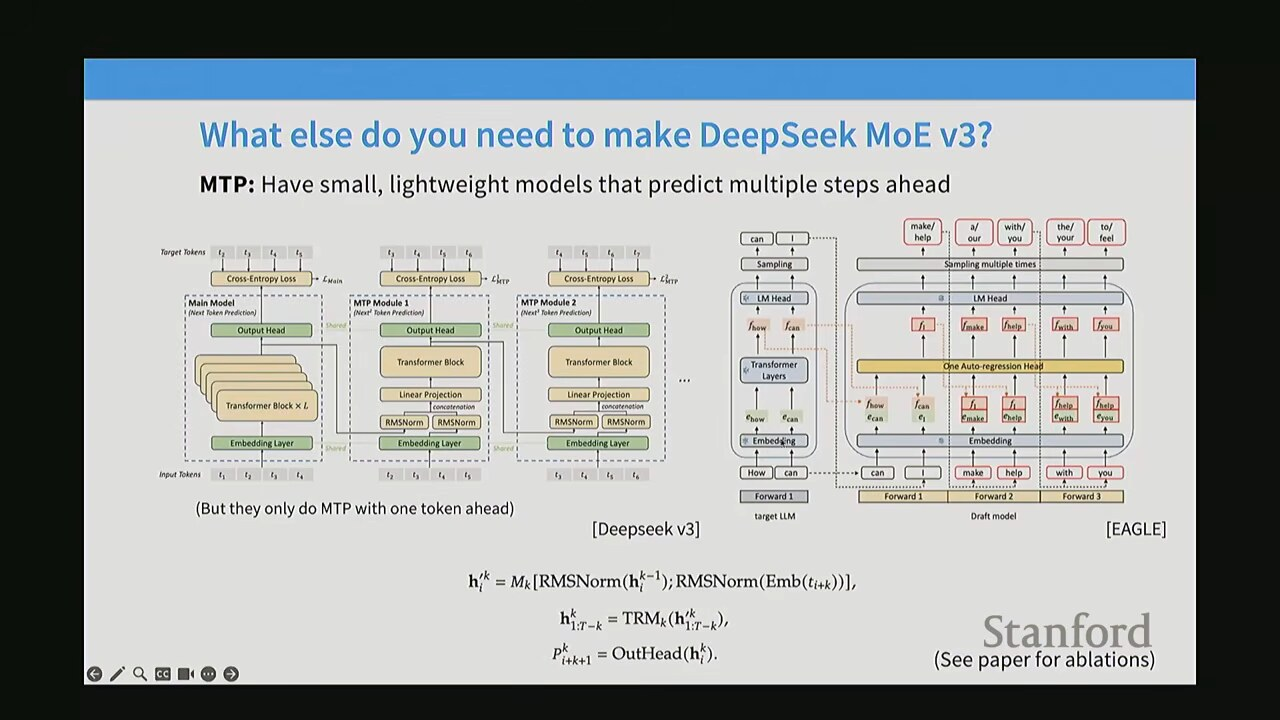
\includegraphics[width=\textwidth]{figures/fig_29_mtp.jpg}
\caption{MTP（Multi-Token Prediction）：额外预测头同时预测第 2 个 token，提供训练信号并可用于推理加速\protect\footnotemark}
\end{figure}
\footnotetext{视频画面时间区间：01:20:15--01:20:45。}

\begin{practicebox}{MTP 的双重价值}
\begin{itemize}
\item \textbf{训练}：多预测一个 token 等价于多一层监督，迫使模型提前规划未来 token，提升表示质量。
\item \textbf{推理}：额外头天然支持 \emph{speculative decoding}（投机解码），一次前向能验证多个候选 token，加速生成。
\end{itemize}
DeepSeek 在实践中只用一个 MTP 头（depth=1），在收益与复杂度间取得平衡。
\end{practicebox}

形式上，给定输入序列，主头在隐状态 $h_t$ 上预测 $P_1(x_{t+1}\mid x_{\le t})$；MTP 头额外预测第 2 个 token：

\[
P_2(x_{t+2}\mid x_{\le t}) \;=\; \mathrm{softmax}\!\bigl(W_{\text{MTP}}\, f(h_t, x_{t+1})\bigr)
\]

\begin{itemize}
\item $f(\cdot)$ 把当前隐状态与已生成的下一 token 融合成 MTP 头的输入。
\item 训练时两项交叉熵相加，让模型在预测当前 token 时就"瞻前顾后"。
\end{itemize}

\section{总结与延伸}

\subsection{MoE 设计要点回顾}

一个现代 MoE 的完整训练目标，是语言建模主损失与若干辅助项的加权和：

\[
\mathcal{L}_{\text{total}} \;=\; \mathcal{L}_{\text{LM}} \;+\; \alpha\,\mathcal{L}_{\text{balance}} \;+\; \gamma\,\mathcal{L}_{z} \;+\; \delta\,\mathcal{L}_{\text{comm}}
\]

\begin{itemize}
\item $\mathcal{L}_{\text{LM}}$：主语言建模损失（next-token prediction 的交叉熵）。
\item $\mathcal{L}_{\text{balance}}$：专家负载均衡损失（Switch 式内积损失）；若用 DeepSeek 的 bias 方案则此项可省或保留极小权重。
\item $\mathcal{L}_{z}$：z-loss，稳定 router softmax。
\item $\mathcal{L}_{\text{comm}}$：通信均衡损失（大规模并行时使用）。
\item $\alpha,\gamma,\delta$：很小的权重系数，需要小心调节——这正是 MoE 训练比 dense 更"娇贵"的根源。
\end{itemize}

\begin{knowledgebox}{本讲核心结论}
\begin{itemize}
\item \textbf{条件计算}是 MoE 的本质：总参数大、单 token 计算量小，解耦"容量"与"算力"。
\item \textbf{Router} 本质是一次 attention 式的内积 + softmax + top-k；token-choice 是主流路由策略。
\item \textbf{Fine-grained + shared expert}（DeepSeek）让专家更专精、通用知识不重复，是当前较优设计。
\item \textbf{负载均衡}是 MoE 训练的生命线：Switch 的辅助损失或 DeepSeek 的 bias-based 无损失均衡，二选其一。
\item \textbf{训练稳定性}靠三件套：均衡机制、z-loss、router 高精度（float32）。
\item \textbf{工程}：expert parallelism + all-to-all 通信、token dropping 控容量、top-M 设备路由压通信。
\item \textbf{DeepSeek V3} 把规模推到 671B/37B，并以 MLA 压 KV cache、MTP 加速，代表了 MoE 路线的 SOTA 工程实践。
\end{itemize}
\end{knowledgebox}

\subsection{开放问题}

\begin{itemize}
\item 最优 router 设计仍是开放问题：线性 router 已足够好，但更优的路由（如可微 routing、专家选择 routing）仍在探索。
\item 专家数、top-k、容量因子的最优配置高度依赖任务与硬件，缺乏普适理论指导。
\item MoE 在微调（尤其到下游小数据任务）时易出现专家利用不均，需要专门策略。
\item 通信开销在大规模下仍是主要瓶颈，未来可能依赖更激进的局部化路由或新的硬件互联。
\end{itemize}

\begin{warningbox}{不要被"稀疏"误导}
"稀疏"并不意味着总能省算力：当专家被分布到多设备、且需要 all-to-all 通信时，通信成本可能反过来主导。评估 MoE 是否真的高效，必须把"专家计算节省"与"通信/调度开销"放在一起算总账。DeepSeek 引入通信均衡损失与 top-M 设备路由，正是为了让这笔回报为正。
\end{warningbox}

\end{document}
